\documentclass[10pt]{article}
\usepackage[utf8]{inputenc}
\usepackage[T1]{fontenc}
\usepackage{hyperref}
\hypersetup{colorlinks=true, linkcolor=blue, filecolor=magenta, urlcolor=cyan,}
\urlstyle{same}
\usepackage{amsmath}
\usepackage{amsfonts}
\usepackage{amssymb}
\usepackage[version=4]{mhchem}
\usepackage{stmaryrd}
\usepackage{caption}
\usepackage{graphicx}
\usepackage[export]{adjustbox}
\graphicspath{ {./images/} }

\title{Terrain Adaptive Trajectory Planning and Tracking on Deformable Terrains }

\author{James Dallas, Michael P. Cole, Paramsothy Jayakumar, and Tulga Ersal}
\date{}


%New command to display footnote whose markers will always be hidden
\let\svthefootnote\thefootnote
\newcommand\blfootnotetext[1]{%
  \let\thefootnote\relax\footnote{#1}%
  \addtocounter{footnote}{-1}%
  \let\thefootnote\svthefootnote%
}

%Overriding the \footnotetext command to hide the marker if its value is `0`
\let\svfootnotetext\footnotetext
\renewcommand\footnotetext[2][?]{%
  \if\relax#1\relax%
    \ifnum\value{footnote}=0\blfootnotetext{#2}\else\svfootnotetext{#2}\fi%
  \else%
    \if?#1\ifnum\value{footnote}=0\blfootnotetext{#2}\else\svfootnotetext{#2}\fi%
    \else\svfootnotetext[#1]{#2}\fi%
  \fi
}

\begin{document}
\maketitle
\captionsetup{singlelinecheck=false}


\begin{abstract}
In this work, a novel single-level adaptive trajectory planner and tracking controller is developed for off-road autonomous vehicles operating on deformable terrains. Trajectory planning and tracking algorithms often rely on a simplified vehicle model to predict future vehicle states based upon control inputs, hence requiring accurate modeling and parameterization. On off-road deformable terrains this is a challenging task due to unknown terrain parameters and the complex interactions at tireterrain interfaces, which pose issues in continuous differentiability, operating conditions, and computational time. To address these difficulties, in this paper, a neural network deformable terrain terramechanics model and its implementation within a terrain adaptive model predictive control algorithm is presented to improve vehicle safety and performance through more accurate prediction of the plant response. It is shown in simulations that the neural network is able to predict the lateral tire forces accurately and efficiently compared to the Soil Contact Model as a state-of-the-art model and is able to yield accurate bicycle model predictions. It is demonstrated that the implementation of the neural network within model predictive control can outperform both a baseline Pacejka-based and a rapidly exploring random tree controller by improving performance and allowing for more severe maneuvers to be completed that otherwise lead to failure when terrain deformations are not explicitly taken into account. The improved performance achieved through estimating terrain parameters online in an adaptive controller is highlighted against the nonadaptive realization. Finally, it is shown the algorithm is conducive to real-time implementation.
\end{abstract}

Index Terms-Adaptive control, autonomous ground vehicles, collision avoidance, model predictive control, terrain estimation, terramechanics, vehicle dynamics, vehicle safety

\section*{I. Introduction}
Military ground vehicles are often required to operate in off-road environments with deformable terrains, where vehicle mobility is significantly impacted by the tire-terrain interaction [1]. As a result, military autonomous ground vehicles (AGVs) must account for these interactions for safe and high-performance navigation. Because common approaches to navigate AGVs rely on model based predictions, it is necessary to model the tire-terrain interaction accurately and efficiently such that AGVs can realize their full potential, even in challenging off-road deformable terrains.

\footnotetext{Manuscript submitted December 15, 2020. Copyright (c) 2015 IEEE. Personal use of this material is permitted. However, permission to use this material for any other purposes must be obtained from the IEEE by sending a request to \href{mailto:pubs-permissions@ieee.org}{pubs-permissions@ieee.org}.

This work was supported by the Automotive Research Center in accordance with Cooperative Agreement W56HZV-19-2-0001 U.S. Army Ground Vehicle Systems Center, Warren, Michigan. (Corresponding author: Tulga Ersal.)\\
J. Dallas and T. Ersal are with the Department of Mechanical Engineering, University of Michigan, Ann Arbor, MI 48109 (e-mail: \href{mailto:dallasja@umich.edu}{dallasja@umich.edu}; \href{mailto:tersal@umich.edu}{tersal@umich.edu}).\\
M.P. Cole and P. Jayakumar are with the U.S. Army Ground Vehicle Systems Center, Warren, MI 48397 (e-mail: michael.p.cole26.civ@army.mil; paramsothy.jayakumar.civ@army.mil).

DISTRIBUTION STATEMENT A. Approved for public release; distribution unlimited. OPSEC \#4662.
}\section*{A. Background}
One approach for AGV trajectory planning and tracking is model predictive control (MPC). MPC has successfully been applied to autonomous navigation for on-road, structured environments [2], [3], [4]. MPC has also been demonstrated for trajectory planning and tracking for static obstacle avoidance in unstructured environments, more representative of off-road military environments, with no lane boundaries or traffic rules to obey [5], [6]. In [7], the results were extended to unstructured environments with moving obstacles. While this research has shown success in obstacle avoidance, the impact of tire-terrain interaction on deformable terrains is not considered [6].

In the off-road domain, nonlinear MPC has been utilized for non-deformable rough terrain navigation [8]. Researchers have also considered information theoretic MPC and model predictive path integral control method for control of a fifth scale Auto-Rally vehicle on an outdoor dirt track [9], [10]. While success has been demonstrated on a dirt track, deformable terrains are not explicitly considered and divergence in learned dynamics could pose safety issues in obstacle avoidance. An MPC tracking controller has also been developed for low speed Martian rover navigation, where MPC is employed for tracking an A* path and low level control [11]. Due to the low speeds of rovers, predictions are based upon linearized kinematic models and linear Bekker-based terramechanics. In higher speed applications encountered in military settings, linearized models can lead to large discrepancies when maximum mobility is desired. Furthermore, infeasible commands can be generated in a decoupled planning and tracking algorithm.

Extending these results to deformable terrains is a challenging task, as state-of-the-art deformable terrain terramechanics models are often limited in terms of dynamic operation, computational complexity, or continuous differentiability [1], [12], [13], [14], [15], [16]. Among existing terramechanics models, Bekker-based models have emerged as perhaps the most widely used [1], [17], [13], [14], [15]. In these models the stresses are calculated over the contact patch between a rigid tire and the deformable terrain, and integrated to obtain the forces acting on the tire [14]. To accurately represent the complex stress distribution generated at the contact patch, Bekker-based models rely on numerous parameters that describe the terrain characteristics, such as cohesion and internal friction angle, to name a few. However, knowledge of these parameters is limited in vehicle operation, where a vehicle may be operating on unknown terrains or terrains in which the properties vary. Furthermore, classical Bekker-based models are often limited in application to steady-state operation [14].

An extension of Bekker's method, known as the Soil Contact Model (SCM), discretizes the tire-terrain interaction and\\[0pt]
allows for dynamic operation [1], [18]. However, due to the discretization and integration of stress, SCM can potentially be too computationally expensive for real-time applications [16]. In response to this limitation, a Bekker-based SCM surrogate model has been developed to extend classical Bekker theory to account for some additional dynamic effects [16]. While the surrogate model developed in [16] proved sufficient for estimation purposes, the lack of twice continuous differentiability poses difficulties when utilized in model-dependent navigation algorithms, such as MPC [6].

As such, a computationally efficient, twice continuously differentiable and dynamic terramechanics model for deformable terrains is still needed for AGV navigation. A potential candidate to address this need is neural networks, which have already demonstrated success in predicting tire forces for onroad applications [19], [20], [21] and in slip detection on deformable terrains [22]; however, extending such approaches to lateral force prediction on deformable terrains is still an open research area. The efficiency and continuous differentiability of neural networks make them a suitable candidate for a terramechanics model in off-road model-dependent navigation architectures. However, such surrogate models will still rely on numerous parameters that characterize the terrain properties that are likely to be unknown a priori and hence need to be estimated online.

As such, a robust MPC navigation strategy must be able to learn terrain properties online and adapt as new information becomes available. With regards to this, terrain adaptive MPC has primarily been considered for navigation in on-road environments [23], [24], [25], [26]. Contingent MPC has shown success in control on icy and snow covered roads [27]. While this prior work begins to address terrain adaptive MPC, it does not consider off-road deformable terrains.

Learning has been combined with control in prior works. For example, in [10] data driven system identification is used for model predictive path integral control of a fifth-scale Auto-Rally vehicle. In [28], a data-driven control approach is developed for optimal tracking for strict-feedback nonlinear systems and demonstrated on a Van der Pol oscillator. A disturbance model is learned in [29] for path tracking using learning-based NMPC that demonstrates success in reducing path-tracking errors at low speed. Finally, a review of learningbased MPC is presented in [30]. However, learning-based MPC is still an open research area for trajectory planning and tracking when maximum mobility is desired on off-road deformable terrains.

\section*{B. Original Contributions}
In light of the literature review above, a gap is identified. Namely, even though MPC has demonstrated success in both known on- and off-road domains, and adapting to road conditions in on-road settings, modeling and adaptation for deformable terrains have not been considered. These limitations are addressed in this work. Specifically, the original contributions of this work are

\begin{enumerate}
  \item a novel neural network deformable terramechanics model satisfying the requirements for use within an MPC framework and its implementation within terrain estimation;
  \item a terrain-adaptive single-level trajectory planning and tracking MPC framework for off-road AGVs operating on deformable terrains; and
  \item high-fidelity simulation based evaluations of the new framework, with comparisons against the state of the art and a nonadaptive realization.\\[0pt]
To this end, first, a neural network deformable terramechanics model is developed. The model allows for dynamic operation on deformable terrain while maintaining sufficient fidelity and satisfying the continuous differentiability requirements of the optimization solver used in MPC. Second, the neural network is integrated with a bicycle model, which serves as the prediction model, and an Unscented Kalman Filter is utilized to estimate the dominant terrain parameter and update this prediction model online. Third, the prediction model and Unscented Kalman Filter are implemented in a single-level nonlinear MPC framework for simultaneous trajectory planning and tracking control. Simulations with a plant represented as an 11 degrees-of-freedom (DoF) military vehicle operating on a clay SCM terrain demonstrate the utility of the framework. To demonstrate the importance of accurately modeling the tire-terrain interactions, the neural network deformable terramechanics model is first benchmarked against an MPC controller that employs the Pacejka model, as Pacejka models have also been demonstrated to be suitable for off-road terrains [31]. A second benchmark compares the MPC controller to rapidly exploring random trees. Then the importance of terrain adaptation is highlighted by comparing a nonadaptive and adaptive neural-network based MPC framework for obstacle avoidance. The outcomes depict the significance of accurately modeling the tire-terrain interaction for safe and high mobility AGVs operating on off-road deformable terrains.
\end{enumerate}

A preliminary version of this work was presented in a conference [32]. The conference paper only presented the MPC formulation for deformable terrains, without any terrain adaptation and without presenting the development of the neural network based terramechanics model. Compared to the conference version, this paper presents 1) the development of the neural network based terramechanics model; 2) the evaluation of the performance of the neural network based terramechanics model against SCM as the state of the art benchmark; 3) the development of the terrain estimator; 4) the evaluation of the terrain estimation performance; 5) the development of the terrain-adaptive MPC framework; and 6) the simulation based evaluation of the new framework against the state of the art and the nonadaptive formulation.

\section*{C. Organization}
The rest of the paper is organized as follows. Sec. II develops the neural network model for deformable terramechanics. Sec. III outlines the MPC framework, including the formulation of cost, constraints, and vehicle dynamics. Sec. IV gives a brief overview of the terrain estimator. Sec. V first describes the simulation setup. Then it demonstrates the utility of the neural network and the improved performance of the developed terrain-adaptive MPC for deformable terrains over Pacejka based and non-adaptive schemes. Finally, Sec. VI gives the conclusions of this study.

\section*{II. Neural Network Terramechanics Model}
In this work, SCM is utilized as the ground truth, generation of the training data for the neural network, and serves as the terramechanics model for the plant model described in Sec. III-B1. An overview of SCM can be found in [17], [12]. Verification of the model can be found in [18], [33]. Briefly, SCM relies on discretization of the terrain and, based upon the deformations at each node, determines relevant stresses that are then integrated to obtain the tire contact force. The stresses are based on the well-known Bekker equations, where the pressure $\sigma$ is expressed as [34]


\begin{equation*}
\sigma=\left(k_{c} / b+k_{\phi}\right) h^{n} \tag{1}
\end{equation*}


and the shear stress $\tau$ is expressed as [35]


\begin{equation*}
\tau=\tau_{\max }\left(1-e^{-j / k}\right) \tag{2}
\end{equation*}


with $\tau_{\text {max }}$ given as


\begin{equation*}
\tau_{\max }=(c+\sigma \tan \phi) \tag{3}
\end{equation*}


where $b$ is the tire effective width, $h$ is the sinkage, $j$ is the deformation, and the remaining variables correspond to terrain parameters where $k_{c}$ is the cohesive modulus, $k_{\phi}$ the frictional modulus, $n$ the sinkage exponent, $k$ the shear deformation modulus, $c$ the cohesion, and $\phi$ the internal friction angle. However, SCM is rather complex and may not be suitable for online application due to the large computational cost [16].

Second, a dynamic Bekker-based surrogate to SCM serves as a comparison between the neural network performance and state-of-the-art approaches. Briefly, the Bekker-based surrogate calculates the stresses as in Eq. (1) to (3); however, functions for $k, j$, and a scaling factor for $\tau_{\text {max }}$ are determined to extend traditional Bekker models to dynamic operation. Once the functions are determined for $k, j$, and $\tau_{\text {max }}$, the lateral forces are obtained through integrating a quadratic approximation of the stresses over the contact patch, where $h$ is determined iteratively by the Newton-Raphson method. The model is then validated with over 1,500 independent simulations to show the generalizability of the model. More information on this surrogate model can be found in [16].

Finally, due to the lack of twice continuous differentiability of this Bekker-based surrogate model, a neural network is developed as the third terramechanics model and as one of the original contributions of the paper. This model is explained further next.

Similar to the Bekker-based surrogate described in [16], the inputs considered for the neural network include the Bekker terrain properties, slip ratio, slip angle, tire velocity, load, and steering rate, because these variables have been demonstrated to impact the force generation at the tire terrain interface. Measurements required to calculate these inputs can be obtained by a global navigation satellite system/global positioning system, an inertial measurement unit, and wheel encoders.

A Latin Hypercube Sampling (LHS) approach maximizing the minimum distance between points of the neural network inputs, with the ranges given in Table I, is used in developing the SCM data set for training the neural network. The input

\begin{table}[h]
\begin{center}
\captionsetup{labelformat=empty}
\caption{TABLE I: Neural network input space.}
\begin{tabular}{|l|l|}
\hline
Input & Range \\
\hline
Slip ratio & -1 to $1(-)$ \\
\hline
Slip angle & -0.6 to 0.6 (rad) \\
\hline
Longitudinal velocity & 2 to $10(\mathrm{~m} / \mathrm{s})$ \\
\hline
Load & 500 to $5500(\mathrm{~N})$ \\
\hline
Steering rate & -0.56 to $0.56(\mathrm{rad} / \mathrm{s})$ \\
\hline
Soil deformation modulus & 43000 to $2080000\left(\mathrm{~N} / \mathrm{m}^{n+1}\right)$ \\
\hline
Sinkage exponent & 0.3 to 1.3 (-) \\
\hline
Shear deformation modulus & 0.01 to 0.024 (m) \\
\hline
Cohesion & 650 to $20700(\mathrm{~Pa})$ \\
\hline
Internal friction angle & 0.105 to 0.66 (rad) \\
\hline
\end{tabular}
\end{center}
\end{table}

ranges are determined from the expected operating range of the vehicle, while the terrain parameter space is compiled from the literature. One difference in the training set is that an aggregate parameter $k^{*}=\left(k_{c} / b+k_{\phi}\right)$ is used for the soil deformation modulus as in [17]. The network targets are generated by propagating the Latin hypercube samples through the SCM terrain implementation in the modeling and simulation software Chrono [36]. Once the data is generated, the data set is split into $70 \%$ training, $15 \%$ validation, and $15 \%$ test sets. Then, the MATLAB Deep Learning toolbox is used to train the network through Bayesian regularization backpropagation, a mean squared error performance function, and hyperbolic tangent sigmoid transfer functions that guarantees twice continuous differentiability, as the neural network is a composition of continuously differentiable functions. The hyperbolic tangent sigmoid transfer function is given as follows:


\begin{equation*}
\operatorname{tansig}(x)=\frac{2}{1+e^{-2 x}}-1 \tag{4}
\end{equation*}


Due to randomness in the weight and bias initialization, 50 neural networks are trained and the network with the best performance is selected as the terramechanics model, where all 50 networks correspond to the description given in the previous paragraph. 2 hidden layers of a total of 14 neurons, with 12 neurons in the first and 2 in the second layer, with approximately 10,000 Latin hypercube samples achieve sufficient performance for the purposes of terrain estimation.

\section*{III. MPC Formulation}
A single-level nonlinear MPC formulation is employed for the purpose of simultaneous trajectory planning and tracking in an environment with static obstacles. The optimal control problem (OCP) formulation is based upon [7], [32] and is given in general form as follows:

\[
\begin{array}{cl}
\underset{\zeta, \xi, t_{f}}{\operatorname{minimize}} & J\left(\zeta(t), \xi(t), \xi\left(t_{f}\right)\right) \\
\text { subject to } & \dot{\xi}(t)=V(\zeta(t), \xi(t), \theta) \\
& \xi_{\min } \leq \xi(t) \leq \xi_{\max } \\
& \zeta_{\min } \leq \zeta(t) \leq \zeta_{\max } \\
& R[\xi(t)] \leq 0 \\
& S[\xi(t)] \leq 0 \tag{10}
\end{array}
\]

In the above expression, $\zeta$ is the vector of control variables, $\xi$ is the vector of states, $\theta$ is a parameter set representing terrain conditions, and $t_{f}$ is the final time. Eq. (5) represents\\
the objective function penalizing the terminal constraints, state evolution, and control effort. Eq. (6) satisfies the nonlinear bicycle model representing the vehicle dynamics. Eq. (7) and (8) are the state and control constraints, respectively. Eq. (9) represents the conditions for reaching the desired terminal vehicle state. Finally, Eq. (10) imposes conditions to satisfy obstacle avoidance. These equations are discussed in detail in the next subsections.

\section*{A. Cost Function}
The cost function is defined as


\begin{align*}
J & =w_{t} t_{f} \\
& +w_{\psi} \int_{t_{0}}^{t_{f}}\left(\sin \left(\psi_{f}\right)\left(x(t)-x_{f}\right)\right. \\
& \left.-\cos \left(\psi_{f}\right)\left(y(t)-y_{f}\right)\right)^{2} d t  \tag{11}\\
& +\int_{t_{0}}^{t_{f}}\left(w_{\dot{\delta}} \dot{\delta}(t)^{2}+w_{J_{x}} J_{x}(t)^{2}\right) d t \\
& +\frac{\sqrt{\left(x\left(t_{f}\right)-x_{f}\right)^{2}+\left(y\left(t_{f}\right)-y_{f}\right)^{2}}}{\sqrt{\left(x\left(t_{0}\right)-x_{f}\right)^{2}+\left(y\left(t_{0}\right)-y_{f}\right)^{2}}+\epsilon}
\end{align*}


where $w_{t}, w_{\psi}, w_{\dot{\delta}}$, and $w_{J_{x}}$ are weightings on the terminal time, desired vehicle heading, and the control variables steering rate and longitudinal jerk, respectively, and $\epsilon$ is a small number that prevents division by zero. The first term seeks to minimize time-to-goal, an important metric in military and racing applications. The second term is a soft constraint such that the vehicle approaches the goal position at the desired heading. The third term penalizes the control effort over the prediction horizon. The final term penalizes the distance of the vehicle's terminal position from the goal position normalized with respect to the distance to the goal at the initial point of the OCP.

\section*{B. Vehicle Models}
\begin{enumerate}
  \item Plant Model: The physical vehicle in the simulationbased validation of the proposed surrogate model, terrain estimator, and MPC formulation is modeled through an 11DoF notional military vehicle with SCM as the terramechanics model in the Chrono software [36]. The vehicle is composed of a double wishbone suspension, rack-pinion steering, 4-wheel drive, and a simple powertrain without a torque converter or transmission [16].
  \item Prediction Model: The vehicle dynamics for MPC predictions, and for predictions in the Unscented Kalman Filter, are represented with a 3-DoF bicycle model, as it has been demonstrated to be of a suitable balance between efficiency and fidelity for short prediction horizons [37]. Therefore, the state vector is given as:
\end{enumerate}

\[
z:=\left[\begin{array}{c}
x  \tag{12}\\
y \\
\psi \\
u \\
v \\
\omega \\
\delta \\
a_{x}
\end{array}\right]=\left[\begin{array}{c}
\text { global } \mathrm{x} \text { position of front axle } \\
\text { global y position of front axle } \\
\text { yaw angle } \\
\text { longitudinal speed } \\
\text { lateral speed } \\
\text { yaw rate } \\
\text { steering angle } \\
\text { longitudinal acceleration }
\end{array}\right]
\]

The state evolution of Eq. (6) is then given by:

\[
\dot{z}(t, n)=\left[\begin{array}{c}
u(t) \cos \psi(t)-\left(v(t)+L_{\mathrm{f}} \omega(t)\right) \sin \psi(t)  \tag{13}\\
u(t) \sin \psi(t)+\left(v(t)+L_{\mathrm{f}} \omega(t)\right) \cos \psi(t) \\
\omega(t) \\
a_{x}(t) \\
\left(F_{\mathrm{yf}}(n)+F_{\mathrm{yr}}(n)\right) / M-u(t) \omega(t) \\
\left(F_{\mathrm{yf}}(n) L_{\mathrm{f}}-F_{\mathrm{yr}}(n) L_{\mathrm{r}}\right) / I_{z z} \\
0 \\
0
\end{array}\right]
\]

In the above expression, $M$ is the vehicle mass, $I_{z z}$ is the moment of inertia, and $L_{\mathrm{f}}$ and $L_{\mathrm{r}}$ are the distances from the center of gravity to the front and rear axles, respectively. $F_{\mathrm{yf}}$ and $F_{\mathrm{yr}}$ are the lateral forces acting on the vehicle body generated by the tires at the front and rear axles, respectively. Two tire models are utilized within the prediction model as explained next.\\
3) Terramechanics Model: For an MPC based trajectory planning and tracking algorithm to successfully complete its task, two considerations about the prediction model must be taken into account. First, since MPC relies on the prediction model to map control inputs to vehicle states, it is required that the prediction model be of sufficient fidelity with respect to the plant. Second, to maintain efficiency in the solver such that real-time implementation can be achieved, twice continuous differentiability of all functions are required. Resulting from these two conditions, it is critical that terramechanics models maintain high fidelity under dynamic conditions while also satisfying the continuous differentiability requirements of the solver.

The neural network deformable terramechanics model of Sec. II satisfies these requirements and is thus employed here to predict $F_{\mathrm{y}(\mathrm{f}, \mathrm{r})}$.

Second, a Pacejka tire model serves as a benchmark to demonstrate the impact of terramechanics model fidelity. The Pacejka model is parameterized from on-road experiments provided by the U.S. Army Ground Vehicle Systems Center for the light-duty military vehicle under study. While the Pacejka model could be parameterized for off-road terrains as in [31], performing such parameterizations is beyond the scope of this study.

\section*{C. State and Control Constraints}
The state constraints of Eq. (7) are given as:

\[
\left[\begin{array}{c}
x_{\min }  \tag{14}\\
y_{\min } \\
\psi_{\min } \\
u_{\min } \\
a_{x, \min }(u(t)) \\
\delta_{\min }
\end{array}\right] \leq\left[\begin{array}{c}
x(t) \\
y(t) \\
\psi(t) \\
u(t) \\
a_{x}(u(t), t) \\
\delta(t)
\end{array}\right] \leq\left[\begin{array}{c}
x_{\max } \\
y_{\max } \\
\psi_{\max } \\
u_{\max } \\
a_{x, \max }(u(t)) \\
\delta_{\max }
\end{array}\right]
\]

where the acceleration constraints $a_{x, \min }(u(t))$ and $a_{x, \text { max }}(u(t))$ are determined to be constants of -2.6 and $1.9 \mathrm{~m} / \mathrm{s}^{2}$, respectively, by following the same procedure described in [6]. The remaining states not given in Eq. (14) are unconstrained.

The control constraints of Eq. (8) are imposed as maximum and minimum bounds on the steering rate $\dot{\delta}$ and longitudinal jerk $J_{x}$ as:

\[
\left[\begin{array}{c}
\dot{\delta}_{\min }  \tag{15}\\
J_{x, \min }
\end{array}\right] \leq\left[\begin{array}{c}
\dot{\delta}(t) \\
J_{x}(t)
\end{array}\right] \leq\left[\begin{array}{c}
\dot{\delta}_{\max } \\
J_{x, \max }
\end{array}\right]
\]

To ensure a collision free trajectory, hard constraints are imposed on the vehicle position $(x, y)$. These constraints, Eq. (10), are given as


\begin{equation*}
\frac{\left(x(t)-x_{\mathrm{obs}}^{i}\right)^{2}}{\left(a^{i}+m\right)^{2}}+\frac{\left(y(t)-y_{\mathrm{obs}}^{i}\right)^{2}}{\left(b^{i}+m\right)^{2}} \geq 1 \tag{16}
\end{equation*}


where, for the $i^{\text {th }}$ obstacle, ( $x_{\text {obs }}^{i}, y_{\text {obs }}^{i}$ ) represents the center position of the enclosing ellipse with $a^{i}$ and $b^{i}$ as the semimajor and semi-minor axes, and $m$ represents a safety margin.

\section*{D. Terminal State Constraints}
Eq. (9) imposes the terminal state constraints such that the terminal vehicle position $\left(x_{t}, y_{t}\right)$ and yaw $\psi_{t}$ are within a prescribed tolerance $\sigma$ of the goal position ( $x_{g}, y_{g}$ ) and yaw $\psi_{g}$. This is expressed as:

\[
\left[\begin{array}{l}
x_{g}-\sigma_{x}  \tag{17}\\
y_{g}-\sigma_{y} \\
\psi_{g}-\sigma_{\psi}
\end{array}\right] \leq\left[\begin{array}{l}
x\left(t_{f}\right) \\
y\left(t_{f}\right) \\
\psi\left(t_{f}\right)
\end{array}\right] \leq\left[\begin{array}{l}
x_{g}+\sigma_{x} \\
y_{g}+\sigma_{y} \\
\psi_{g}+\sigma_{\psi}
\end{array}\right]
\]

The remaining terminal states are unconstrained.

\section*{E. Solving the OCP}
The OCP is implemented in NLOptControl [38], [39] and solved with IPOPT [40]. NLOptControl performs the translation from continuous to discrete time using Legendre-GaussRadau (LGR) collocation and Gaussian-Legendre quadrature, as described in detail in [39]. In addition, NLOptControl automatically performs the differentiation required to calculate the Jacobian and Hessian, exploiting sparsity in the Hessian through reverse automatic differentiation with the acycliccoloring method that is faster than the star-coloring method [41]. Direct collocation is preferred, as shooting methods face challenges with a large number of variables, and multiple shooting methods require expensive integration at each iteration and can lead to reduced sparsity. On the other hand, direct collocation leads to a larger problem, but preserves sparsity and directly incorporates state constraints at each collocation point. Within NLOptControl, h, p, and hp methods are implemented; however, for this work the hp-method based on LGR collocation is utilized, as it helps prevent inaccuracies of h -methods and large problem sizes of p-methods [41]. Further details and comparisons of NLOptControl to other optimal control software packages are given in [41].

\section*{IV. Terrain Estimation}
The parameter to be estimated is chosen as the sinkage exponent $n$, because the sinkage exponent is the dominant terrain parameter [16], [17]. To estimate the sinkage exponent, an Unscented Kalman filter (UKF) is employed, a detailed implementation of which is given in [16] and a high-level overview is given here for completeness as follows.

Suppose a system is given as:


\begin{align*}
\dot{z}(t) & =F(z(t), \rho(t))  \tag{18}\\
y(t) & =H(z(t), \gamma(t)) \tag{19}
\end{align*}


where $z(t)$ is the augmented state given by the first six states of Eq. (12) appended with additional states, one for each tire, with trivial dynamics representing the sinkage exponent. The process and observation noise are given as $\rho$ and $\gamma$, respectively. $z(t)$ is obtained through forward Euler integration of $F(z(t), \rho(t))$, and $H(z(t), \gamma(t))$ is the measurement model, which is given as the original state vector of the first six states of Eq. (12). The measurements are obtained by corrupting the plant model of Sec. III-B1 with Gaussian noise as described in Sec. V, while the prediction model given by the first six states of Eq. (13) relies on the neural network to predict the lateral forces. In other words, the prediction model is the bicycle model that obtains the lateral forces from the neural network, and the measurements are obtained from the state vector of the 11 DoF plant acting on an SCM terrain in Chrono.

To propagate the previous state distribution to the current state, a number of Sigma Points $Z$ are generated that capture the statistical distribution of the previous state. Applying Eq. (18) to $Z$ yields the transformation of $Z$ to the current state. Effectively, this transformation provides the time evolution of the statistics, i.e., the current mean state $\hat{z}^{-}$and covariance matrix $P^{-}$.

Then, the UKF updates the current state and covariance estimate with current measurements, $y(t)$, as follows:


\begin{align*}
& \hat{z}(t)=\hat{z}^{-}(t)+K(y(t)-\hat{y}(t))  \tag{20}\\
& P(t)=P^{-}(t)-K P_{\hat{y}(t) \hat{y}(t)} K^{T} \tag{21}
\end{align*}


where $\hat{z}(t)$ is the measurement corrected state estimate, $P(t)$ is the updated covariance matrix, $K$ is the Kalman gain, $\hat{y}(t)$ is the predicted value of the measurements based upon the propagation of the state from the previous to current time, and $P_{\hat{y}(t) \hat{y}(t)}$ is the covariance matrix corresponding to $\hat{y}(t)$.

Intuitively, the UKF compares the output of the prediction model (Eq. (18)) with measurements to determine the best estimate of the state. By doing so, the UKF estimates the sinkage exponent that improves the bicycle model's predictive capability as compared to the measurements. A more detailed discussion of the UKF implementation can be found in [42], [16].

The UKF terrain estimator runs in parallel with MPC and updates the MPC prediction model parameters with the current best terrain estimate each time MPC is called, i.e., upon initialization of MPC after the plant has simulated the entire execution horizon.

\section*{V. Results and Discussion}
\section*{A. Neural Network Terramechanics Model and Terrain Estimation}
In this section, the performances of the neural network terramechanics model and the UKF estimator are evaluated. Evaluation is performed on two fronts: 1) the ability of the terramechanics model and UKF estimator to accurately predict

\begin{table}[h]
\begin{center}
\captionsetup{labelformat=empty}
\caption{TABLE II: Terrain parameters for the simulated terrain [14].}
\begin{tabular}{ccc}
\hline
Parameter & Symbol & Clay \\
Cohesive modulus & $k_{c}$ & $13200\left(\mathrm{~N} / \mathrm{m}^{n+1}\right)$ \\
Frictional modulus & $k_{\phi}$ & $692200\left(\mathrm{~N} / \mathrm{m}^{n+2}\right)$ \\
Sinkage exponent & $n$ & $0.5(-)$ \\
Shear deformation modulus & $k$ & $0.01(\mathrm{~m})$ \\
Cohesion & $c$ & $4140(\mathrm{~Pa})$ \\
Internal friction angle & $\phi$ & $0.2269(\mathrm{rad})$ \\
\hline
\end{tabular}
\end{center}
\end{table}

\begin{table}[h]
\begin{center}
\captionsetup{labelformat=empty}
\caption{TABLE III: Measurement standard deviations used for sensor simulation.}
\begin{tabular}{cc}
\hline
State & Noise $(\sigma)$ \\
$x$ & $1.2(\mathrm{~m})$ \\
$y$ & $1.2(\mathrm{~m})$ \\
$\psi$ & $0.0175(\mathrm{rad})$ \\
$u$ & $0.25(\mathrm{~m} / \mathrm{s})$ \\
$v$ & $0.25(\mathrm{~m} / \mathrm{s})$ \\
$\omega_{z}$ & $0.0175(\mathrm{rad} / \mathrm{s})$ \\
\hline
\end{tabular}
\end{center}
\end{table}

tire forces and the sinkage exponent, respectively, and 2 ) the impact these estimated parameters have on improving the prediction capability of the 3-DoF vehicle model. The first evaluation provides insight into the performance of the neural network in predicting tire forces and of the UKF in estimating terrain parameters, while the second provides an assessment of the estimation algorithm's utility for use in MPC schemes.

As an example comparison of the neural network against SCM, the single wheel test bed is used to sweep the tire through a range of slip angles where the load is held constant at 5000 N , the speed is $8.5 \mathrm{~m} / \mathrm{s}$, slip ratio is 0.5 , and the terrain is sand. Hence, this produces the common lateral force vs. slip angle curve. The results of SCM and the neural network are shown in Fig. 1. While it is evident that the neural network matches SCM well for the single wheel test bed, it is of more interest to observe the neural network's performance as the vehicle operates. This is further discussed next.

To maintain consistency and a fair comparison with the terramechanics model developed in [16], the same clay Chrono simulation is used in the evaluation studies. Briefly, the simulation is performed with the 11 DoF plant model of Sec. III-B1 operating on a clay-like SCM terrain. The parameters used in

\begin{figure}[h]
\begin{center}
  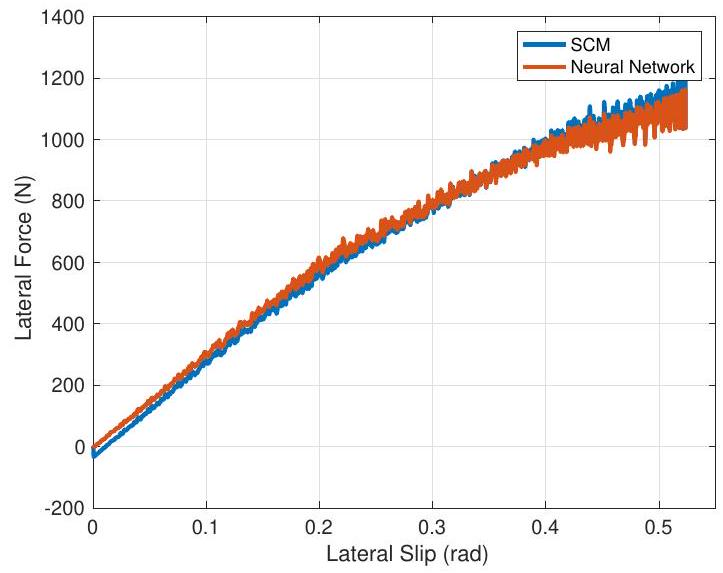
\includegraphics[alt={},max width=\textwidth]{3c87ead7-70d5-42cb-a3a2-ed4cbdde9fd3-06_573_723_1933_216}
\captionsetup{labelformat=empty}
\caption{Fig. 1: Neural Network and SCM output on a sand terrain for a load of 5000 N , slip ratio of 0.5 , and speed of $8.5 \mathrm{~m} / \mathrm{s}$.}
\end{center}
\end{figure}

\begin{table}[h]
\begin{center}
\captionsetup{labelformat=empty}
\caption{TABLE IV: Performance comparison between neural network and Bekkerbased SCM surrogate model in terms of estimated value of and estimation errors in the sinkage exponent $n$ on clay terrain. Bekker-based SCM surrogate results are from [16].}
\begin{tabular}{ccccc}
\hline
Model & Initial guess & True val. & Est. val. & $\%$ Error \\
Bekker based [16] & 0.7 & 0.5 & 0.519 & $3.8 \%$ \\
Neural network & 0.7 & 0.5 & 0.505 & $1 \%$ \\
\hline
\end{tabular}
\end{center}
\end{table}

\begin{figure}[h]
\begin{center}
  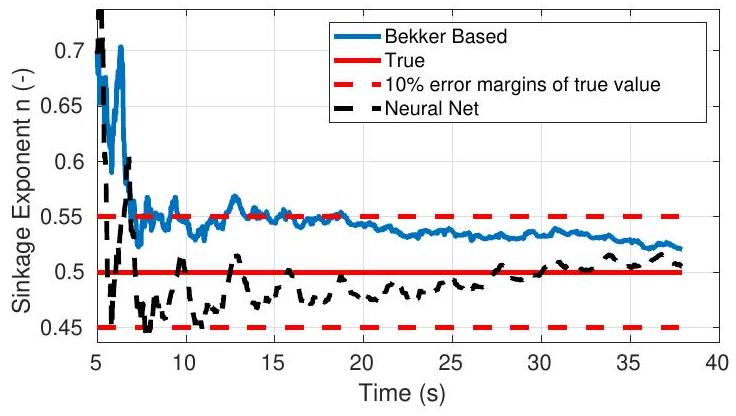
\includegraphics[alt={},max width=\textwidth]{3c87ead7-70d5-42cb-a3a2-ed4cbdde9fd3-06_416_736_541_1125}
\captionsetup{labelformat=empty}
\caption{Fig. 2: Simulated sinkage exponent estimation for neural network based terramechanics model (black dashed line) and Bekker-based model of [16] (blue solid line).}
\end{center}
\end{figure}

representing the clay terrain are given in Table II. The vehicle is then subjected to sinusoidal steering commands, steering fully in both directions, and sinusoidal throttle commands such that varying speed is achieved. Once the simulation completes, the measurement data is generated by corrupting the state vector with additive noise, with standard deviations given in Table III. More information on the simulation settings and the steering and velocity profiles can be found in [16].

Table IV summarizes the estimation results, including the initial guess, true sinkage exponent used by Chrono's SCM, along with the UKF estimated value and the percent error for the Bekker-based SCM surrogate of [16] and the neural network terramechanics model. Here, the estimated value is taken to be the converged value at the end of the simulation. For both terramechanics models the UKF estimator performs relatively well and estimates the parameter within $4 \%$ of its true value. However, as shown in Fig. 2, the UKF that uses the neural network reduces estimation error after 19 s of simulation time, i.e., once the estimator has converged within $10 \%$ of the true value, by over $87 \%$ as compared to [16] on average over the remaining simulation time. Also, the neural network (black dashed line) converges faster compared to the model of [16] (blue solid line); i.e., within $10 \%$ accuracy at 11 s vs. 19 s . This improvement in convergence speed could prove beneficial in time critical applications, e.g., collision imminent steering. These findings suggest that, between the bicycle models using the two terramechanics models, the one in conjunction with the neural network is preferred for terrain estimation, since it can achieve a higher level of estimation accuracy as compared to the bicycle model relying on the Bekker-based surrogate of [16] while also converging at a faster rate and having the beneficial property of twice continuous differentiability. While the UKF does not require calculation of the Jacobian, and hence does not require the neural network, the same prediction model should be used by

\begin{figure}[h]
\begin{center}
  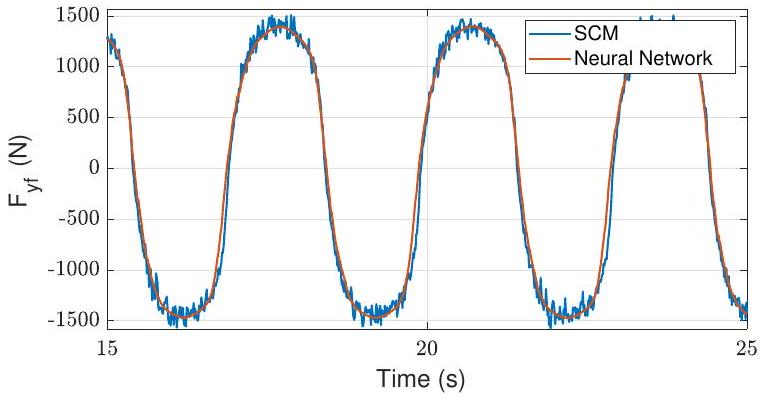
\includegraphics[alt={},max width=\textwidth]{3c87ead7-70d5-42cb-a3a2-ed4cbdde9fd3-07_399_764_268_193}
\captionsetup{labelformat=empty}
\caption{Fig. 3: Simulated SCM and neural network lateral forces from estimation on a clay terrain.}
\end{center}
\end{figure}

\begin{figure}[h]
\begin{center}
  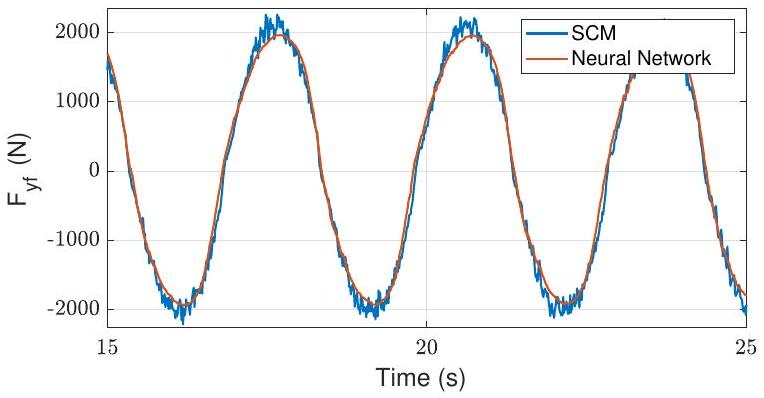
\includegraphics[alt={},max width=\textwidth]{3c87ead7-70d5-42cb-a3a2-ed4cbdde9fd3-07_398_764_915_193}
\captionsetup{labelformat=empty}
\caption{Fig. 4: Simulated SCM and neural network lateral forces from estimation on a sandy loam terrain.}
\end{center}
\end{figure}

both the UKF and MPC to prevent a discrepancy in the best estimates that could arise from the separate prediction models.

Fig. 3 shows the lateral forces from the front tire acting on the vehicle body given by SCM and the neural network running within the estimator. The forces predicted by the neural network are reasonable as compared to SCM with a root-mean-squared-error (RMSE) of 109 N . These forces are obtained from the sinusoidal vehicle simulation on clay, as discussed at the beginning of this section, and hence are completely different data than that generated by LHS in training the neural network. As such, the good agreement observed in Fig. 3 suggests the network is able to generalize beyond its training and can potentially be applied to an MPC scheme. Fig. 4 shows the lateral forces for a sinusoidal simulation on a sandy loam terrain, demonstrating the force prediction accuracy on multiple terrains. The sandy loam simulation setup is based on [16] and the details can be found therein.

The peak computational time for a single UKF iteration of the bicycle model using the neural network terramechanics model is 6.9 ms , whereas the peak computation time for the bicycle model using the Bekker-based surrogate is 10.5 ms on 16 GB Memory and a single core 3 GHz Intel Core i7 processor running MATLAB R2017a [16]. An optimized C++ version of UKF for the bicycle model using the neural network has a peak computation time of 0.15 ms . The estimator calls the bicycle model 17 times per UKF step, meaning the bicycle

\begin{figure}[h]
\begin{center}
  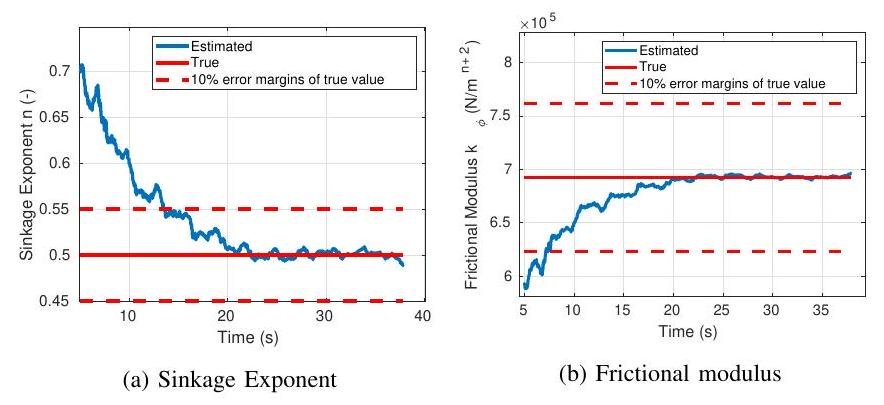
\includegraphics[alt={},max width=\textwidth]{3c87ead7-70d5-42cb-a3a2-ed4cbdde9fd3-07_405_884_193_1069}
\captionsetup{labelformat=empty}
\caption{Fig. 5: Simultaneous estimation of sinkage exponent and frictional modulus for clay sinusoidal simulation.}
\end{center}
\end{figure}

\begin{table}[h]
\begin{center}
\captionsetup{labelformat=empty}
\caption{TABLE V: Mean squared error over entire simulation with 2.5 second prediction horizon for neural network and Bekker SCM surrogate.}
\begin{tabular}{|l|l|l|l|l|}
\hline
Model & \multicolumn{2}{|c|}{Neural Network} & \multicolumn{2}{|c|}{SCM Surrogate [16]} \\
\hline
State & $\mathrm{n}=0.505$ & $\mathrm{n}=0.7$ & $\mathrm{n}=0.519$ & $\mathbf{n} \boldsymbol{=} \mathbf{0 . 7}$ \\
\hline
$x(\mathrm{~m})^{2}$ & 0.033 & 0.045 & 0.037 & 0.01 \\
\hline
$y(\mathrm{~m})^{2}$ & 0.067 & 0.42 & 0.022 & 0.15 \\
\hline
$\psi(\mathrm{rad})^{2}$ & $6.5 \mathrm{e}-04$ & 0.035 & $2.45 \mathrm{e}-04$ & 0.0089 \\
\hline
$u(\mathrm{~m} / \mathrm{s})^{2}$ & $1.33 \mathrm{e}-04$ & $1.33 \mathrm{e}-04$ & $1.33 \mathrm{e}-04$ & $1.33 \mathrm{e}-04$ \\
\hline
$v(\mathrm{~m} / \mathrm{s})^{2}$ & 0.0068 & 0.496 & 0.0047 & 0.15 \\
\hline
$\omega_{z}(\mathrm{rad} / \mathrm{s})^{2}$ & 0.0016 & 0.078 & $9.01 \mathrm{e}-04$ & 0.023 \\
\hline
\end{tabular}
\end{center}
\end{table}

model, and neural network, can be evaluated efficiently and are conducive to real-time applications.

As a second analysis of the UKF, in addition to solely estimating the sinkage exponent, the frictional modulus is estimated simultaneously, as the these two parameters exhibit the highest sensitivity. The results are shown in Fig. 5, demonstrating the ability of the UKF to accurately estimate multiple parameters simultaneously. While the UKF is able to estimate multiple parameters simultaneously, and results are shown to demonstrate this capability, the focus of this work relates to solely estimating the most sensitive parameter, $n$, in an MPC setting. Estimating multiple parameters, identifiability of parameters, and the trade off of the increased computational load that results from estimating multiple parameters as compared to improved predictive capabilities are subject to future work.

As such, the results favor the accuracy, computational efficiency, and twice continuous differentiability of the neural network over the Bekker based model of [16].

To assess the applicability of the proposed UKF estimator and neural network terramechanics model for predictive applications, the bicycle model, with the neural network parameterized by the converged estimates, is used to predict the vehicle states approximately 2.5 s into the future. This is chosen to mimic the procedure used by MPC and follows the same evaluation process as in [16] to allow comparisons.

Table V gives the mean squared error (MSE) over the entire clay simulation with 2.5 s predictions for the bicycle model utilizing the neural network terramechanics model and the model reported in [16] for both the initial guess and converged value of the sinkage exponent. The baseline for this error calculation is the 11-DoF Chrono simulation. Utilizing the converged sinkage exponent for the neural network signifi-

\begin{figure}[h]
\begin{center}
  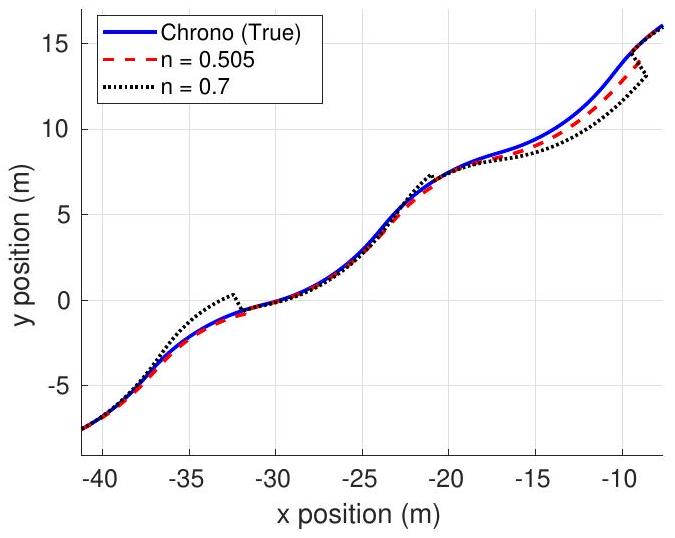
\includegraphics[alt={},max width=\textwidth]{3c87ead7-70d5-42cb-a3a2-ed4cbdde9fd3-08_538_675_227_247}
\captionsetup{labelformat=empty}
\caption{Fig. 6: Chrono simulation for an AGV on SCM clay terrain with true vehicle positions from Chrono (blue solid line), bicycle model parameterized by $n=$ 0.505 (red dashed line), and bicycle model parameterized by initial terrain guess $n=0.7$ (black dotted line) over an approximately 2.5 s prediction horizon.}
\end{center}
\end{figure}

\begin{table}[h]
\begin{center}
\captionsetup{labelformat=empty}
\caption{TABLE VI: Obstacle settings for simulation Scenarios 1 and 2 [32].}
\begin{tabular}{cccc}
\hline
Obstacle & Location & Radius & Safety Margin \\
Scen. 1: Obs. 1 & $(0 \mathrm{~m}, 2 \mathrm{~m})$ & 3 m & 1 m \\
Scen. 2: Obs. 1 & $(-10 \mathrm{~m}, 2.5 \mathrm{~m})$ & 3 m & 1 m \\
Scen. 2: Obs. 2 & $(0.1 \mathrm{~m},-2.5 \mathrm{~m})$ & 3 m & 1 m \\
\hline
\end{tabular}
\end{center}
\end{table}

cantly reduces the MSE in the state prediction as compared to the initial guess, in some cases by an order of magnitude. Comparing the state errors associated with the converged sinkage exponent for the neural network and the Bekkerbased surrogate, it can be seen that the errors of the neural network are slightly larger than that of the Bekker-based surrogate; however, the errors for the neural network are still reasonable, achieving position prediction RMSEs on the order of 25 cm over a 2.5 second horizon. These results suggest that the neural network terramechanics model can be suitable for estimation and is better suited for application in control due to its accuracy, increased efficiency and twice continuous differentiability. Furthermore, the reduction in prediction error achieved through the estimated parameters can potentially yield better performing model predictive navigation and control.

The increased performance of the bicycle model utilizing the estimated terrain parameter with the neural network terramechanics model is depicted in Fig. 6. The position predictions of the bicycle model for the estimated terrain parameter $n=0.505$ (red dashed line) are much closer ( 0.26 m RMSE in $y$ deviation as compared to Chrono) to the true Chrono simulation (blue solid line) as compared to using the initial guess $n=0.7$ ( 0.65 m RMSE in $y$ deviation as compared to Chrono) for the sinkage exponent (black dotted line). It is anticipated that this improved position accuracy can be beneficial to autonomous obstacle avoidance using MPC. Assessing this expected benefit systematically is discussed next.

\section*{B. Terrain-Adaptive Obstacle Avoidance}
To assess the utility of the terramechanics model and estimator in an MPC scheme, three scenarios are considered. The first two scenarios motivate the need for a deformable terrain terramechanics model as compared to an on-road Pacejka model, while the third scenario depicts the utility of online terrain estimation. In all scenarios, the 11-DoF notional lightduty military vehicle operating on a clay SCM terrain in Chrono acts as the plant [36]. The clay terrain parameters are given in Table II. For the UKF, the states reported from the plant are corrupted with random additive Gaussian noise, with the standard deviations given in Table III, to simulate sensors. Sensor measurements are updated every 24 ms .

In all scenarios, two prediction models are compared. In Scenarios 1 and 2, which are presented in [32] and are included for completeness, the MPC prediction model is given by the bicycle model of Eq. (13) with $F_{\mathrm{y}(\mathrm{f}, \mathrm{r})}$ predicted by either the Pacejka or the neural network terramechanics model. The controllers corresponding to these two models are denoted as P-MPC and NN-MPC, respectively. For these two scenarios, the terrain parameters for the neural network terramechanics model are set to the nominal values. In Scenario 3, the bicycle model of Eq. (13) utilizes the neural network terramechanics model for both prediction models; however, in one case the neural network utilizes an initial guess for the sinkage exponent, whereas in the other case the sinkage exponent is estimated and updated online based upon the UKF. All other terrain parameters are assumed to have their nominal values given in Table II. This represents a realistic scenario, where terrain classification can be used to determine the terrain class such as in [43], [44] and set nominal values for the specific class, and then terrain identification can be used to hone in on the actual terrain parameters. For this scenario, the controllers in comparison are denoted as IG-MPC and UKFMPC for the controller using only the initial terrain guess and the terrain adaptive controller, respectively. For all scenarios, a 0.5 s execution horizon and a variable prediction horizon based upon time-to-goal is used [6], [7].

In the UKF-MPC, the terrain estimator runs in parallel with the MPC algorithm and adaptation occurs as discussed in Sec. IV.

\begin{enumerate}
  \item Scenario 1: Scenario 1 corresponds to a single obstacle avoidance, with obstacle information given in Table VI, that exhibits a simple maneuver for the vehicle.
\end{enumerate}

While this maneuver can be completed by both the NNMPC and P-MPC, as depicted by the plant path in Fig. 7, the impact of the tire model becomes apparent. In particular, the NN-MPC initiates a more drastic turn early in the maneuver and then steers back towards the centerline prior to passing the obstacle. On the other hand, the P-MPC turns later in the maneuver and continues to drift past the obstacle prior to turning back in towards the centerline. The difference in the plant response is because the plant acts in an under-responsive manner for the P-MPC case. The Pacejka model predicts larger lateral forces for a given input than is achievable by the plant, leading to less drastic steering commands and hence an underresponse of the plant.

\begin{figure}[h]
\begin{center}
  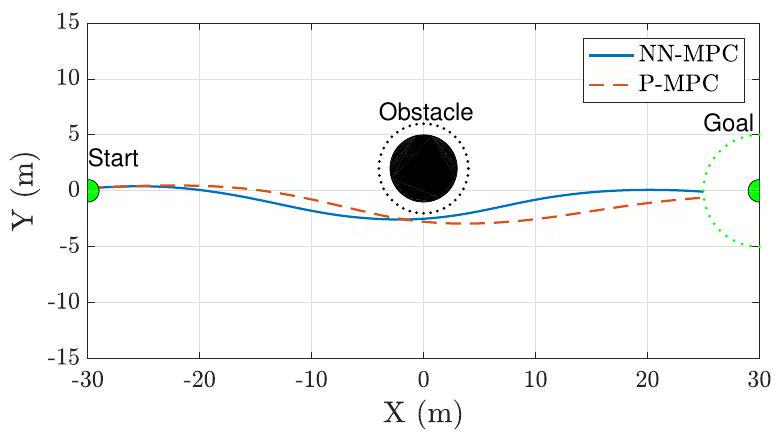
\includegraphics[alt={},max width=\textwidth]{3c87ead7-70d5-42cb-a3a2-ed4cbdde9fd3-09_437_781_184_208}
\captionsetup{labelformat=empty}
\caption{Fig. 7: Plant response to neural network based controller NN-MPC (blue) and Pacejka based controller P-MPC (orange dashed line) for Scenario 1 [32]. Start and goal positions are in green while obstacles and safety margin are given by black disks and black dotted circles, respectively. The green dotted line around the goal represents the tolerance $\sigma$ on the terminal position.}
\end{center}
\end{figure}

\begin{figure}[h]
\begin{center}
  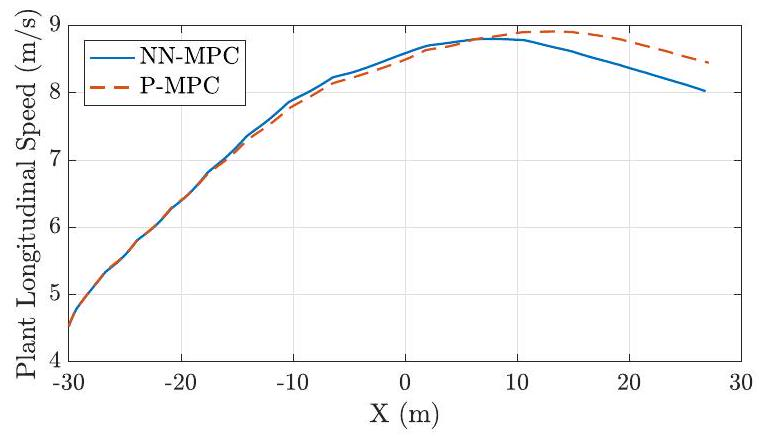
\includegraphics[alt={},max width=\textwidth]{3c87ead7-70d5-42cb-a3a2-ed4cbdde9fd3-09_437_762_846_227}
\captionsetup{labelformat=empty}
\caption{Fig. 8: Plant longitudinal speed for neural network based controller NN-MPC (blue) and Pacejka based controller P-MPC (orange dashed line) for Scenario 1 [32].}
\end{center}
\end{figure}

The difference in the paths becomes important when considering the performance metrics and formulation of the OCP. The more drastic initial turn of the NN-MPC allows for the vehicle to turn back towards the centerline earlier and hence realign to better reach the target state. This is due to Eq. (11), which penalizes the deviation from the centerline and the terminal state, in particular the second term of the cost. A measure of the deviation from the centerline can be taken as the integrated absolute area of the deviation from the centerline, which is 55.5 and $78.2 \mathrm{~m}^{2}$ for the NN-MPC and P-MPC, respectively. Finally the difference between the goal and terminal $y$ position of the plant is 0.07 and 0.6 m for the NN-MPC and P-MPC, respectively, suggesting the NN-MPC can better achieve the goal position than the P-MPC. The time-to-goal is 10.2 s for both controllers, in accordance with the similar longitudinal speed profiles in Fig. 8. Finally, as seen in Fig. 9, a much smoother steering command is observed for the NN-MPC (blue) than the P-MPC (orange). The improved fidelity of the neural network terramechanics model reduces the prediction error as compared to the Pacejka model. Therefore, the terminal state at the end of the execution horizon for the prediction model better replicates that of the plant, leading to less correction required on the control inputs. Hence, while both controllers complete the maneuver in similar time, NNMPC demonstrates improved performance as compared to P MPC in generating smooth steering commands, minimizing terminal $y$ position, and reducing deviation from centerline.

\begin{figure}[h]
\begin{center}
  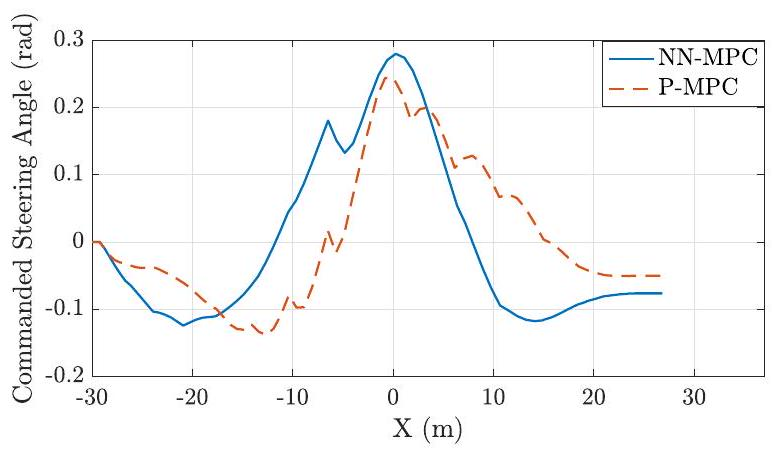
\includegraphics[alt={},max width=\textwidth]{3c87ead7-70d5-42cb-a3a2-ed4cbdde9fd3-09_450_772_184_1117}
\captionsetup{labelformat=empty}
\caption{Fig. 9: Commanded steering angle for neural network based controller NNMPC (blue) and Pacejka based controller P-MPC (orange dashed line) for Scenario 1 [32].}
\end{center}
\end{figure}

\begin{figure}[h]
\begin{center}
  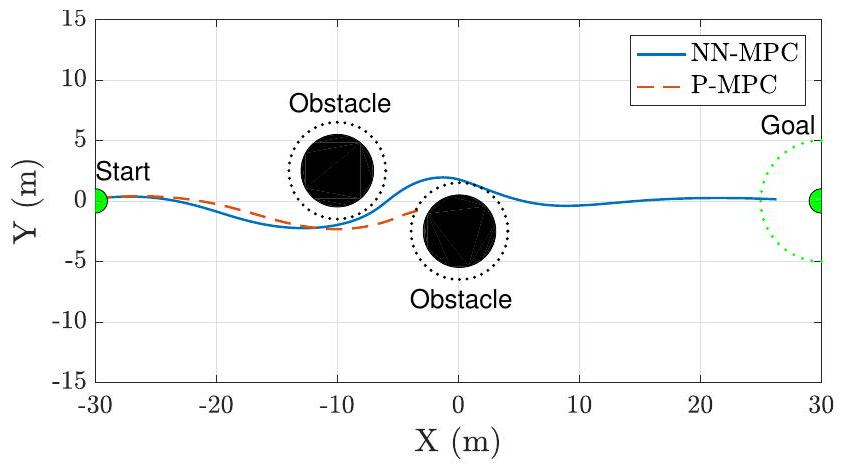
\includegraphics[alt={},max width=\textwidth]{3c87ead7-70d5-42cb-a3a2-ed4cbdde9fd3-09_467_843_784_1110}
\captionsetup{labelformat=empty}
\caption{Fig. 10: Plant response to neural network based controller NN-MPC (blue) and Pacejka based controller P-MPC (orange dashed line) for Scenario 2 [32]. Start and goal positions are in green while obstacles and safety margin are given by black disks and black dotted circles, respectively. The green dotted line around the goal represents the tolerance $\sigma$ on the final position. Overlap of NN-MPC and second obstacle's safety margin is an artifact of line thickness and does not result from collision.}
\end{center}
\end{figure}

These results suggest that despite the discrepancy in the prediction models, the feedback nature of MPC is robust enough for both formulations to complete the maneuver. However, as is shown in the next subsection, this may not be the case in more severe maneuvers.\\
2) Scenario 2: To exhibit a more severe maneuver, two circular objects are placed to force the vehicle through a narrow corridor that requires a high level of fidelity of the prediction model for the vehicle to successfully navigate. The locations of the obstacles are given in Table VI.

The plant response to the two controllers is given in Fig. 10. Again, the P-MPC exhibits the under-responsive behavior of Scenario 1; however, due to the narrow margin of error in this scenario, the controller is unable to recover from the plant prediction model mismatch, ultimately leading to a collision with the second obstacle. On the other hand, the NN-MPC initially turns wide early in the maneuver followed by a sharp turn to avoid the second obstacle, allowing for successful completion of the maneuver. The under-responsive behavior is also evident from Fig. 11, which shows the PMPC controller commands a smaller steering angle than the NN-MPC controller.

Finally, Fig. 13 depicts the longitudinal speed profile of the plant. The NN-MPC initially accelerates from $x$ position of -30 m to -20 m , then decelerates until the vehicle reaches 0

\begin{figure}[h]
\begin{center}
  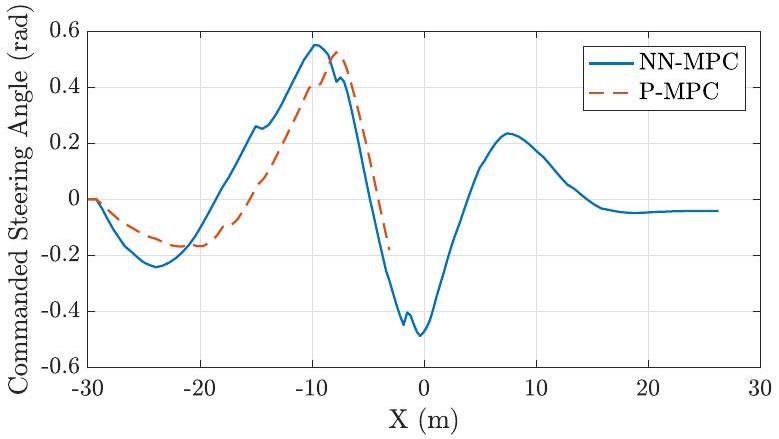
\includegraphics[alt={},max width=\textwidth]{3c87ead7-70d5-42cb-a3a2-ed4cbdde9fd3-10_439_779_193_208}
\captionsetup{labelformat=empty}
\caption{Fig. 11: Commanded plant steering angle for neural network based controller NN-MPC (blue) and Pacejka based controller P-MPC (orange dashed line) for Scenario 2 [32].}
\end{center}
\end{figure}

\begin{figure}[h]
\begin{center}
  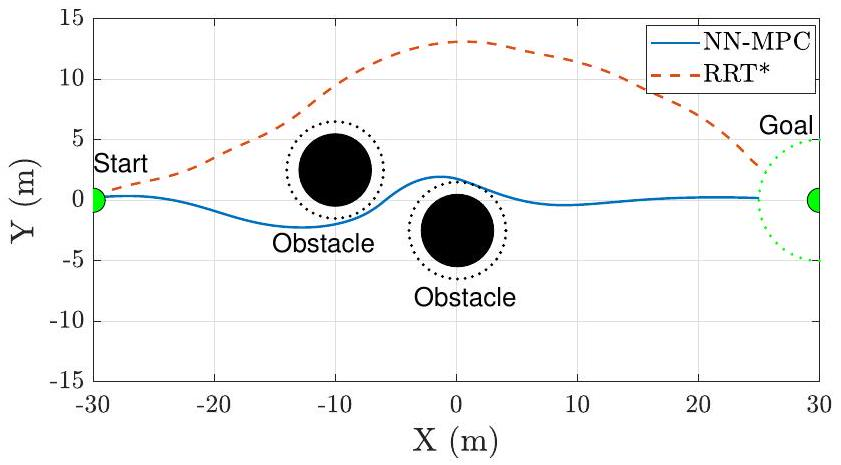
\includegraphics[alt={},max width=\textwidth]{3c87ead7-70d5-42cb-a3a2-ed4cbdde9fd3-10_465_841_786_199}
\captionsetup{labelformat=empty}
\caption{Fig. 12: response to neural network based controller NN-MPC (blue) and RRT* (orange dashed line) for Scenario 2. Start and goal positions are in green, while obstacles and safety margin are given by black disks and black dotted circles, respectively. The green dotted line around the goal represents the tolerance $\sigma$ on the final position. Overlap of NN-MPC and second obstacle's safety margin is an artifact of line thickness and does not result from collision.}
\end{center}
\end{figure}

m , and finally accelerates until the vehicle reaches the goal. The commanded vehicle acceleration is due to the cost on the time-to-goal, which forces the vehicle to accelerate if possible. In the case of the deceleration from -20 m to 0 m , the decrease in the speed shifts weight to the front tires, which allows for larger lateral forces to be generated from the front tire steering. Additionally, the decreased speed allows for more time for the vehicle to maneuver around the obstacles in this challenging area. Once the vehicle is in a position to clear the obstacles, NN-MPC again commands the vehicle to accelerate.

As another comparison to state-of-the-art planners, the same simulation is run using rapidly exploring random trees (RRT*) as the planner. For this simulation, the plant is commanded to have a constant speed of $6 \mathrm{~m} / \mathrm{s}$, which is near the top speed of the NN-MPC simulation, and Chrono's built in steering and speed controllers are used for path following. Fig. 12 shows the plant response for NN-MPC (blue) and RRT* (orange dashed line). RRT* deviates from the NN-MPC path significantly and commands a path that goes wide around the obstacles, as RRT* has no notion of the cost used in MPC. This leads to an integrated deviation from the centerline of 44.71 and $443.65 \mathrm{~m}^{2}$ for NN-MPC and RRT*, respectively. The terminal $y$ position error for NN-MPC is 0.18 m and 2.6 m for RRT*. Finally, consistent with RRT* having a higher average speed, the time-to-goal for RRT* is 13.4 s , whereas the time-to-goal

\begin{figure}[h]
\begin{center}
  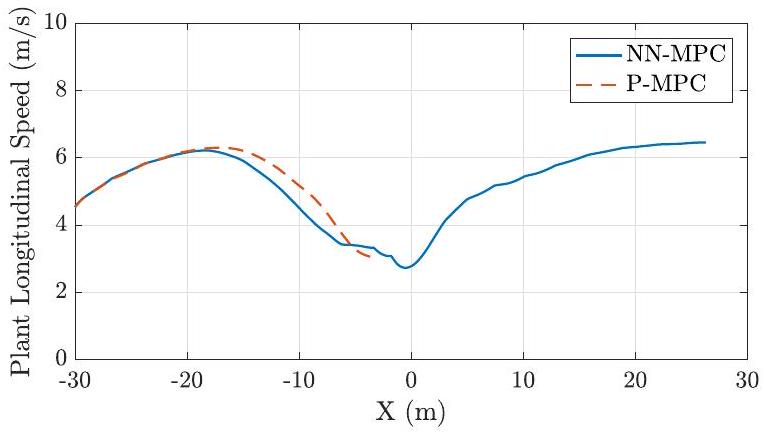
\includegraphics[alt={},max width=\textwidth]{3c87ead7-70d5-42cb-a3a2-ed4cbdde9fd3-10_433_764_201_1134}
\captionsetup{labelformat=empty}
\caption{Fig. 13: Plant longitudinal speed response to neural network based controller NN-MPC (blue) and Pacejka based controller P-MPC (orange dashed line) for Scenario 2 [32].}
\end{center}
\end{figure}

\begin{table}[h]
\begin{center}
\captionsetup{labelformat=empty}
\caption{TABLE VII: LHS input range for Scenario 3.}
\begin{tabular}{ccc}
\hline
Input & Min & Max \\
Obstacle 1 Position $(\mathrm{x}, \mathrm{y})$ & $(-15,-7)$ & $(-1,7)$ \\
Obstacle 2 Position $(\mathrm{x}, \mathrm{y})$ & $(1,-7)$ & $(15,7)$ \\
Obstacle Radius & 0.5 & 3 \\
Sinkage Exponent $(\mathrm{n})$ & 0.4 & 1.0 \\
\hline
\end{tabular}
\end{center}
\end{table}

for NN-MPC is 14.5 s .\\
3) Scenario 3: In this scenario, the vehicle must avoid two obstacles to assess the utility of the terrain estimator. Unlike the first two scenarios, a Monte Carlo simulation is conducted in this case with variations in obstacle radii and locations as well as initial guess for the sinkage exponent. To determine the number of samples necessary to obtain statistically significant results, $G^{*}$ Power is used with a paired sample t-test, effect size of 0.5 , significance level of 0.05 , and a power of 0.8 , giving a total of 27 samples [45]. Then, LHS is used to determine the positions and radii of the two obstacles, along with the initial guess for the sinkage exponent. The LHS input range is given in Table VII, with the samples maximizing the minimum distance between points.

The IG-MPC assumes no estimation takes place and hence fixes the sinkage exponent to the initial guess, while UKFMPC estimates the sinkage exponent and updates the prediction model as the simulation runs. Ultimately, the scenario assesses the utility of the estimator to improve prediction model fidelity and its impact in an MPC setting. Due to the location of the obstacles, the estimator converges to within $10 \%$ of the true terrain parameter in only 8 of the 27 cases. This is because the obstacle locations, generated by LHS, often do not force the vehicle to induce significant dynamics for sinkage exponent identification, i.e., there is no persistent excitation. In cases where the estimator does not converge, the estimated value still approaches the true terrain parameter as compared to the initial guess.

An example of a case from the simulations where the estimator fails to converge to the true value is shown in Fig. 14 and 15. As seen in Fig. 15, the estimator starts at an initial guess for the sinkage exponent of 0.9 and approaches the true value until the $x$ position reaches -10 m , at which point the estimator appears to stabilize around a value of 0.65 . In comparing with the vehicle position of Fig. 14, the vehicle is turning in avoidance of the first obstacle until an $x$

\begin{figure}[h]
\begin{center}
  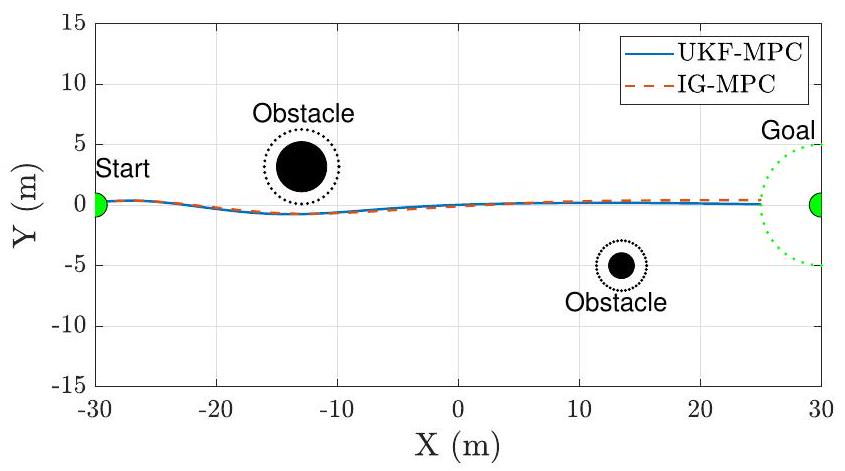
\includegraphics[alt={},max width=\textwidth]{3c87ead7-70d5-42cb-a3a2-ed4cbdde9fd3-11_471_845_180_197}
\captionsetup{labelformat=empty}
\caption{Fig. 14: Plant response to UKF-MPC (blue) and IG-MPC (orange dashed line) for a case without persistent excitation in Scenario 3. Start and goal positions are in green while obstacles and safety margin are given by black disks and black dotted circles, respectively. The green dotted line around the goal represents the tolerance on the final position.}
\end{center}
\end{figure}

\begin{figure}[h]
\begin{center}
  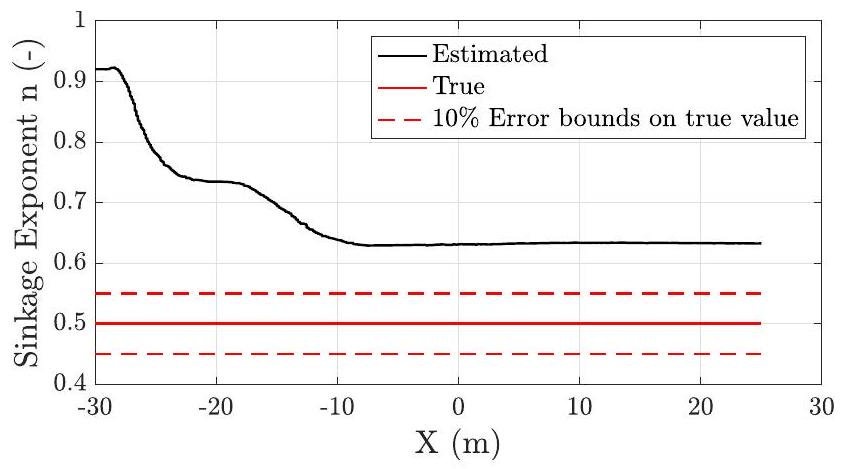
\includegraphics[alt={},max width=\textwidth]{3c87ead7-70d5-42cb-a3a2-ed4cbdde9fd3-11_469_845_861_197}
\captionsetup{labelformat=empty}
\caption{Fig. 15: Estimated sinkage exponent for the case in Fig. 14 is shown in black. True sinkage exponent is shown as red solid line and $10 \%$ error bounds on the true value are shown as red dashed lines.}
\end{center}
\end{figure}

position of about -10 m , after which the vehicle drives along the centerline until the goal is reached. Thus it is apparent that the estimator is approaching the true terrain parameter when the vehicle is maneuvering around the first obstacle, but once the vehicle passes the first obstacle, the induced lateral dynamics are insufficient for the estimator to gain meaningful information, relating to lack of persistent excitation. If the lateral force acting on the vehicle is zero, no estimation can take place, as the impact of the terrain parameter on the vehicle response enters through the lateral force $F_{\mathrm{y}(\mathrm{f}, \mathrm{r})}$.

Fig. 16 and 17 demonstrate one of the LHS simulations where the estimator converges to the true terrain parameter. As seen in Fig. 16, the maneuver is more challenging than the case of Fig. 14, requiring the vehicle to deviate from the centerline to avoid the obstacles. This more challenging maneuver causes the controller to command a more drastic steering input, shown in Fig. 18, hence inducing sufficient lateral dynamics for estimation.

In comparing the UKF-MPC to IG-MPC, Fig. 16 shows that both controllers follow a similar path, but the UKF-MPC turns more aggressively back towards the centerline near the end of the maneuver, reducing the cost associated with the second term of Eq. (11). This causes the integrated absolute area of the deviation from the centerline to be 104.4 and $117.05 \mathrm{~m}^{2}$ for the UKF-MPC and IG-MPC, respectively. The terminal $y$ position error of the vehicle is 1.39 m and 2.34 m for the

\begin{figure}[h]
\begin{center}
  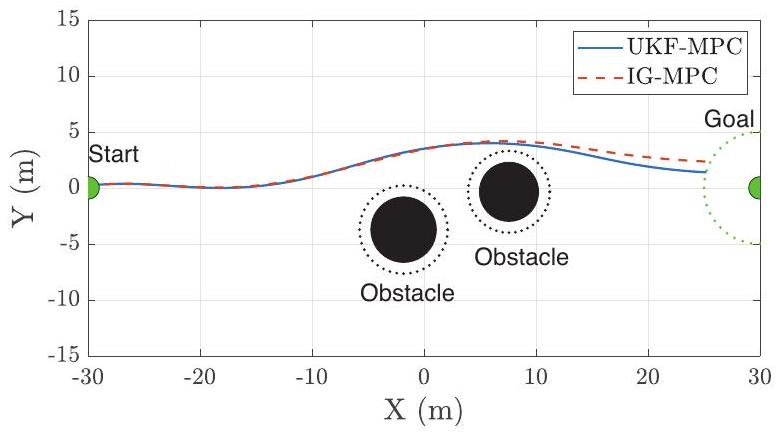
\includegraphics[alt={},max width=\textwidth]{3c87ead7-70d5-42cb-a3a2-ed4cbdde9fd3-11_435_781_195_1121}
\captionsetup{labelformat=empty}
\caption{Fig. 16: Plant response to UKF-MPC (blue) and IG-MPC (orange dashed line) for a case with persistent excitation in Scenario 3. Start and goal positions are in green while obstacles and safety margin are given by black disks and black dotted circles, respectively. The green dotted line around the goal represents the tolerance on the final position.}
\end{center}
\end{figure}

\begin{figure}[h]
\begin{center}
  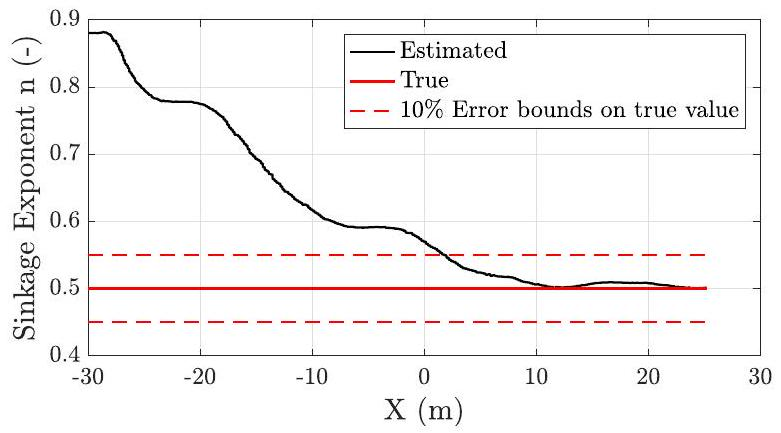
\includegraphics[alt={},max width=\textwidth]{3c87ead7-70d5-42cb-a3a2-ed4cbdde9fd3-11_433_781_850_1121}
\captionsetup{labelformat=empty}
\caption{Fig. 17: Estimated sinkage exponent for the case in Fig. 16 is shown in black. True sinkage exponent is shown as red solid line and $10 \%$ error bounds on the true value are shown as red dashed lines.}
\end{center}
\end{figure}

UKF-MPC and IG-MPC, respectively. This is due to an underresponsive plant in the IG-MPC case, which commands a smaller magnitude steering angle input than the UKF-MPC as shown in Fig. 18. Additionally, both UKF-MPC and IG-MPC follow a similar commanded speed profile as shown in Fig. 19, but UKF-MPC commands a slightly larger longitudinal speed. This leads to a time-to-goal of 10.28 s and 10.49 s for the UKF-MPC and IG-MPC, respectively.

Finally, in all 27 simulations, both IG-MPC and UKF-MPC are able to successfully complete the maneuver, but UKFMPC significantly outperforms IG-MPC in two performance metrics. Various performance metrics, representative of terms

\begin{figure}[h]
\begin{center}
  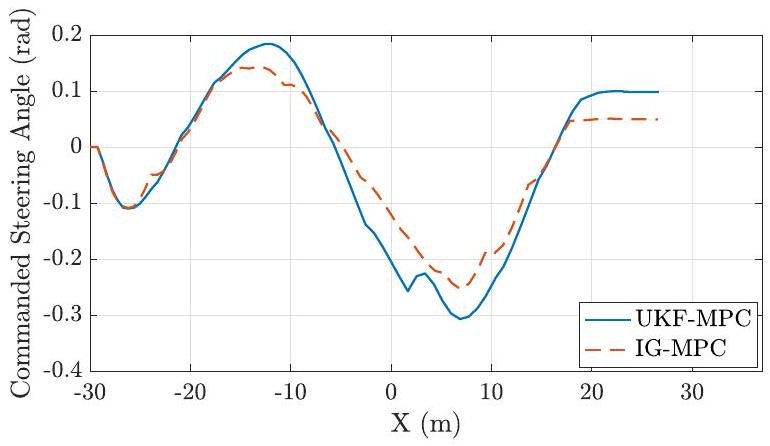
\includegraphics[alt={},max width=\textwidth]{3c87ead7-70d5-42cb-a3a2-ed4cbdde9fd3-11_446_770_2066_1119}
\captionsetup{labelformat=empty}
\caption{Fig. 18: Commanded plant steering angle for UKF-MPC (blue) and IG-MPC (orange dashed line) for the case in Fig 16.}
\end{center}
\end{figure}

\begin{figure}[h]
\begin{center}
  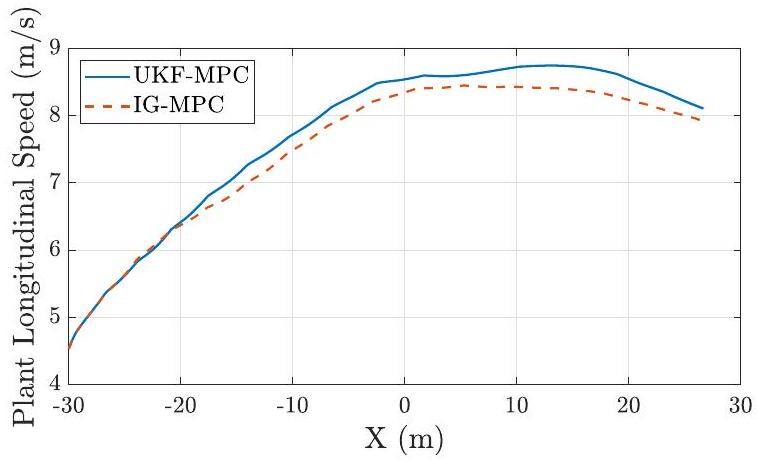
\includegraphics[alt={},max width=\textwidth]{3c87ead7-70d5-42cb-a3a2-ed4cbdde9fd3-12_463_757_197_227}
\captionsetup{labelformat=empty}
\caption{Fig. 19: Plant longitudinal speed response to UKF-MPC (blue) and IG-MPC (orange dashed line) for the case in Fig 16.}
\end{center}
\end{figure}

\begin{table}[h]
\begin{center}
\captionsetup{labelformat=empty}
\caption{TABLE VIII: IPOPT solve times for each scenario [32].}
\begin{tabular}{ccc}
\hline
Case & Mean & Peak \\
Scenario 1: P-MPC & 0.11 s & 0.15 s \\
Scenario 1: NN-MPC & 0.28 s & 0.44 s \\
Scenario 2: NN-MPC & 0.26 s & 0.35 s \\
Scenario 3: IG-MPC & 0.35 s & 0.6 s \\
Scenario 3: UKF-MPC & 0.35 s & 0.59 s \\
\hline
\end{tabular}
\end{center}
\end{table}

in Eq. (11), are shown in Fig. 20 for IG-MPC and UKFMPC. These metrics are compared for statistically significant difference using the Analysis of Variance (ANOVA) with a significance level of $5 \%$; i.e., if the p value resulting from ANOVA is $p<0.05$, then the null hypothesis that there is no statistically significant difference between the metrics is rejected with $95 \%$ confidence, implying that utilizing the estimator makes an impact. Based on this analysis, significant improvement is achieved by UKF-MPC as compared to IGMPC in integrated absolute deviation area from the centerline ( $p<0.001$ ) and terminal $y$ position ( $p<0.01$ ), corresponding to the second term of Eq. (11). In the case of time-to-goal ( $p>0.1$ ) and mean solve time ( $p>0.1$ ), no noticeable improvement is observed. This is likely because the controller does not force the vehicle to diverge between different routes, leading to similar time-to-goal between UKF-MPC and IGMPC. Finally, in terms of the time integral of the absolute steering rate, the UKF-MPC induces a significantly larger cost in the third term of Eq. (11) as compared to IG-MPC ( $p<0.0001$ ), as the steering rate is the trade-off of improved centerline tracking.

These results suggest that despite both IG-MPC and UKFMPC being able to successfully complete the 27 maneuvers, the improved prediction fidelity of UKF-MPC improves performance of the autonomous navigation algorithm. A sample size much larger than 27 is needed to determine the edge cases similar to Scenario 2, where the difference between the two formulations manifests itself not only in performance but also safety. Such an investigation is subject to future research and needs to overcome the computational expense of the plant simulations.\\
4) Computational Performance: Table VIII reports the mean and peak solve times for each scenario and controller on an Intel Xeon E-2176G 3.7 GHz processor and 16 GB RAM. In the case that the vehicle is unable to complete\\
the maneuver, no solve time is reported. The reported solve times exclude spikes in solve time, e.g. when IPOPT returns restoration failure. However, the peak solve times of each simulation often occur at iterations near the spikes, e.g., at the iteration after a restoration failure. In such cases control commands from previous MPC iterations are applied. Such spikes occur infrequently, approximately $5 \%$ of the MPC iterations, and occur for both the Pacejka and neural network model, suggesting the errors are not necessarily a result of the terramechanics model.

As seen in Table VIII, when controllers are able to successfully complete the maneuver, the peak solves times are less than the execution horizon, resulting in real-time capability. On average, NN-MPC demands roughly 2.5 times more computational cost than the P-MPC, which is the trade-off against the higher fidelity terramechanics model. No noticeable difference in computational cost is observed between the UKF-MPC and IG-MPC of Scenario 3.

Despite the increased solve time of the NN-MPC, the higher fidelity improves performance (Scenario 1 and 2) and safety (Scenario 2). In addition, UKF-MPC improves performance at no noticeable increase in computational cost (Scenario 3 ). Thus these results favor the adaptive neural network terramechanics model in situations where vehicles operate near mobility limits, such as off-road military applications. Finally, the speed range of these simulations are consistent with the current expected operating range for off-road AGVs, which is $5 \mathrm{~m} / \mathrm{s}$ for complex terrain and $10 \mathrm{~m} / \mathrm{s}$ for open terrain, as set by the RACER program of the US Defense Advanced Research Projects Agency (DARPA).

\section*{VI. Conclusion}
This work develops a novel terrain-adaptive MPC framework for simultaneous trajectory planning and tracking for AGVs operating on off-road deformable terrains. The novelty is in the development of neural network terramechanics modeling for dynamic operation and its utilization within terrain estimation and the MPC prediction model, along with the utilization of terrain adaptation in MPC. These two contributions allow for more accurate force prediction during trajectory planning and tracking on deformable terrains. It is shown that the neural network achieves comparable accuracy to state-of-the-art dynamic terramechanics models while reducing the peak computation time. The results suggest the neural network terramechanics model is able to predict tire lateral forces with sufficient accuracy for the problem of terrain estimation and control. It is demonstrated that the neural network in combination with a UKF leads to comparable accuracy in sinkage exponent estimation as compared to state-of-the-art methods while also satisfying the differentiability requirements of optimal control and offering reduced computational time. It is demonstrated that the estimated terrain parameters can significantly reduce the prediction errors of a 3-DoF bicycle model when the neural network terramechanics model is parameterized according to the estimated sinkage exponent. Therefore, it is concluded that the neural network terramechanics model and its implementation within the estimator are an important advancement toward off-road AGVs.

\begin{figure}[h]
\begin{center}
  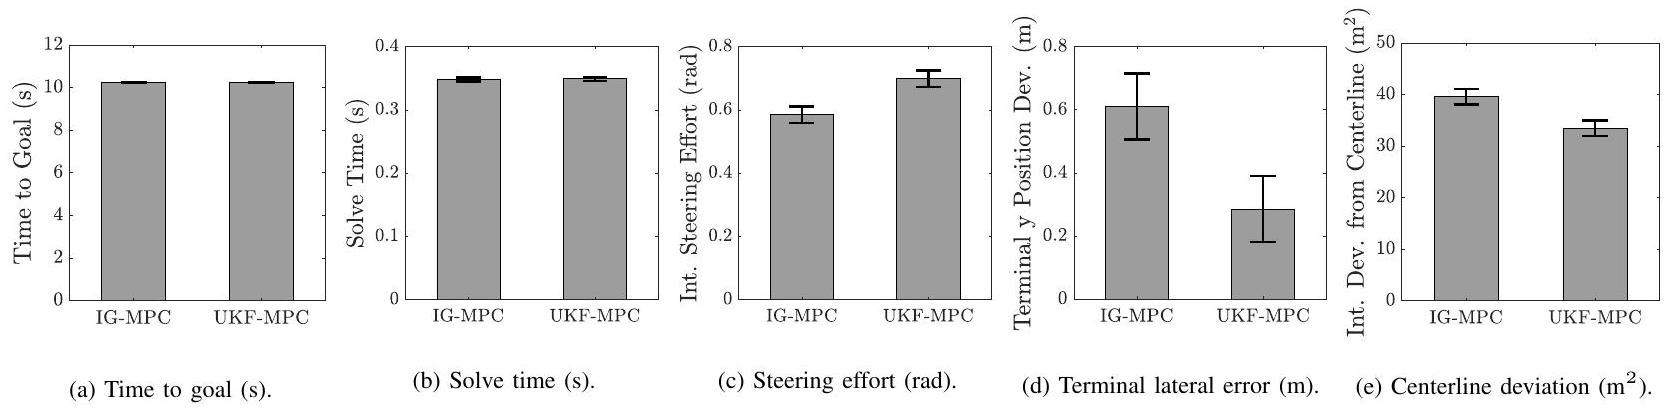
\includegraphics[alt={},max width=\textwidth]{3c87ead7-70d5-42cb-a3a2-ed4cbdde9fd3-13_411_1670_195_225}
\captionsetup{labelformat=empty}
\caption{Fig. 20: Performance metrics for Scenario 3 of mean value and standard error of mean difference.}
\end{center}
\end{figure}

The utility of the neural network terramechanics model is then demonstrated in MPC, where it is shown that the model improves performance and safety of MPC while also remaining computationally efficient by satisfying the differentiability requirements of the optimizer. It is shown that this expands the AGV operational domain. Furthermore, the utility of terrain estimation is highlighted in an MPC setting, demonstrating improved performance metrics through achieving higher fidelity prediction models as compared to the plant. Therefore, it is concluded that the developed terrainadaptive MPC framework for simultaneous trajectory planning and tracking is an important step in enabling high mobility AGVs operating on off-road deformable terrains.

Future work considers extending the algorithm to rough, 3D terrains. It is also of interest to experimentally validate the algorithm. Formally evaluating the stability properties of the developed MPC formulation is also identified as in important future research direction.

\section*{References}
[1] S. Taheri, C. Sandu, S. Taheri, E. Pinto, and D. Gorsich, "A technical survey on terramechanics models for tire-terrain interaction used in modeling and simulation of wheeled vehicles," Journal of Terramechanics, vol. 57, pp. 1-22, 2015.\\[0pt]
[2] J. Nilsson, P. Falcone, M. Ali, and J. Sjöberg, "Receding horizon maneuver generation for automated highway driving," Control Engineering Practice, vol. 41, pp. 124-133, 2015.\\[0pt]
[3] J. V. Frasch, A. Gray, M. Zanon, H. J. Ferreau, S. Sager, F. Borrelli, and M. Diehl, "An auto-generated nonlinear MPC algorithm for realtime obstacle avoidance of ground vehicles," in European Control Conference, 2013, pp. 4136-4141.\\[0pt]
[4] A. Gray, Yiqi Gao, T. Lin, J. K. Hedrick, H. E. Tseng, and F. Borrelli, "Predictive control for agile semi-autonomous ground vehicles using motion primitives," in American Control Conference, 2012, pp. 42394244.\\[0pt]
[5] J. Liu, P. Jayakumar, J. L. Stein, and T. Ersal, "A nonlinear model predictive control formulation for obstacle avoidance in high-speed autonomous ground vehicles in unstructured environments," Vehicle System Dynamics, vol. 56, no. 6, pp. 853-882, 2018.\\[0pt]
[6] -, "Combined speed and steering control in high speed autonomous ground vehicles for obstacle avoidance using model predictive control," IEEE Transactions on Vehicular Technology, vol. 66, no. 10, pp. 87468763, 2017.\\[0pt]
[7] H. Febbo, J. Liu, P. Jayakumar, J. L. Stein, and T. Ersal, "Moving obstacle avoidance for large, high-speed autonomous ground vehicles," in American Control Conference, 2017, pp. 5568-5573.\\[0pt]
[8] A. Eick and D. Bevly, "Nonlinear model predictive controller for an unmanned ground vehicle on variable terrain," in ASME Dynamic Systems and Control Conference, 2015.\\[0pt]
[9] G. Williams, N. Wagener, B. Goldfain, P. Drews, J. M. Rehg, B. Boots, and E. A. Theodorou, "Information theoretic MPC for model-based reinforcement learning," in IEEE International Conference on Robotics and Automation, 2017, pp. 1714-1721.\\[0pt]
[10] G. Williams, P. Drews, B. Goldfain, J. M. Rehg, and E. A. Theodorou, "Aggressive driving with model predictive path integral control," in IEEE International Conference on Robotics and Automation, 2016, pp. 14331440.\\[0pt]
[11] G. Binet, R. Krenn, and A. Bemporad, "Model predictive control applications for planetary rovers," in International Symposium on Artificial Intelligence and Robotics in Space, 2012.\\[0pt]
[12] R. Krenn and A. Gibbesch, "Soft Soil Contact Modeling Technique for Multi-Body System Simulation." Springer, Berlin, Heidelberg, 2011, pp. 135-155.\\[0pt]
[13] G. Ishigami, A. Miwa, K. Nagatani, and K. Yoshida, "Terramechanicsbased model for steering maneuver of planetary exploration rovers on loose soil," Journal of Field Robotics, vol. 24, no. 3, pp. 233-250, 2007.\\[0pt]
[14] W. C. Smith, "Modeling of wheel-soil interaction for small ground vehicles operating on granular soil," Ph.D. dissertation, University of Michigan, 2014.\\[0pt]
[15] T. Guo, "Power consumption models for tracked and wheeled small unmanned ground vehicles on deformable terrains," Ph.D. dissertation, University of Michigan, 2016.\\[0pt]
[16] J. Dallas, K. Jain, Z. Dong, L. Sapronov, M. P. Cole, P. Jayakumar, and T. Ersal, "Online terrain estimation for autonomous vehicles on deformable terrains," Journal of Terramechanics, vol. 91, pp. 11-22, 2020.\\[0pt]
[17] A. Gallina, R. Krenn, M. Scharringhausen, T. Uhl, and B. Schäfer, "Parameter Identification of a Planetary Rover Wheel-Soil Contact Model via a Bayesian Approach," Journal of Field Robotics, vol. 31, no. 1, pp. 161-175, 2014.\\[0pt]
[18] R. Krenn and G. Hirzinger, "SCM - A soil contact model for multibody system simulations," in European Regional Conference of the International Society for Terrain-Vehicle Systems, Bremen, 2009.\\[0pt]
[19] M. Acosta and S. Kanarachos, "Tire lateral force estimation and grip potential identification using Neural Networks, Extended Kalman Filter, and Recursive Least Squares," Neural Computing and Applications, vol. 30, no. 11, pp. 3445-3465, 2018.\\[0pt]
[20] H. Kim and P. I. Ro, "A Tire Side Force Model by Artificial Neural Network," in International Congress and Exposition, Detroit, MI, 1995.\\[0pt]
[21] J. Matuško, I. Petrović, and N. Perić, "Neural network based tire/road friction force estimation," Engineering Applications of Artificial Intelligence, vol. 21, no. 3, pp. 442-456, 2008.\\[0pt]
[22] R. Gonzalez, D. Apostolopoulos, and K. Iagnemma, "Slippage and immobilization detection for planetary exploration rovers via machine learning and proprioceptive sensing," Journal of Field Robotics, vol. 35, no. 2, pp. 231-247, 2018.\\[0pt]
[23] M. Jalalmaab, M. Pirani, B. Fidan, and S. Jeon, "Cooperative road condition estimation for an adaptive model predictive collision avoidance control strategy," in IEEE Intelligent Vehicles Symposium, 2016, pp. 1072-1077.\\[0pt]
[24] B.-C. Chen, B.-C. Luan, and K. Lee, "Design of lane keeping system using adaptive model predictive control," in IEEE International Conference on Automation Science and Engineering, 2014, pp. 922-926.\\[0pt]
[25] P. Falcone, F. Borrelli, J. Asgari, H. E. Tseng, and D. Hrovat, "Predictive Active Steering Control for Autonomous Vehicle Systems," IEEE Transactions on Control Systems Technology, vol. 15, no. 3, pp. 566580, 2007.\\[0pt]
[26] F. Borrelli, P. Falcone, T. Keviczky, J. Asgari, and D. Hrovat, "MPCbased approach to active steering for autonomous vehicle systems," International Journal of Vehicle Autonomous Systems, vol. 3, no. 2/3/4, p. 265, 2005.\\[0pt]
[27] J. P. Alsterda, M. Brown, and J. C. Gerdes, "Contingency model predictive control for automated vehicles," American Control Conference, pp. 717-722, 2019.\\[0pt]
[28] W. Gao and Z.-P. Jiang, "Learning-based adaptive optimal tracking control of strict-feedback nonlinear systems," IEEE Transactions on Neural Networks and Learning Systems, vol. 29, no. 6, pp. 2614-2624, 2018.\\[0pt]
[29] C. J. Ostafew, A. P. Schoellig, T. D. Barfoot, and J. Collier, "Learning-based nonlinear model predictive control to improve vision-based mobile robot path tracking," Journal of Field Robotics, vol. 33, no. 1, pp. 133-152, 2016. [Online]. Available: \href{https://onlinelibrary.wiley.com/doi/abs/10.1002/rob}{https://onlinelibrary.wiley.com/doi/abs/10.1002/rob}. 21587\\[0pt]
[30] L. Hewing, K. P. Wabersich, M. Menner, and M. N. Zeilinger, "Learning-based model predictive control: Toward safe learning in control," Annual Review of Control, Robotics, and Autonomous Systems, vol. 3, no. 1, pp. 269-296, 2020. [Online]. Available: \href{https://doi.org/10.1146/annurev-control-090419-075625}{https://doi.org/10.1146/annurev-control-090419-075625}\\[0pt]
[31] B. Maclaurin, "Using a modified version of the magic formula to describe the traction/slip relationships of tyres in soft cohesive soils," Journal of Terramechanics, vol. 52, pp. 1-7, 2014.\\[0pt]
[32] J. Dallas, Y. Weng, and T. Ersal, "Combined trajectory planning and tracking for autonomous vehicles on deformable terrains," in ASME Dynamic Systems and Control Conference, 2020.\\[0pt]
[33] A. Gallina, R. Krenn, and B. Schäfer, "On the treatment of soft soil parameter uncertainties in planetary rover mobility simulations," Journal of Terramechanics, vol. 63, pp. 33-47, 2016.\\[0pt]
[34] M. G. Bekker, Theory of Land Locomotion. Ann Arbor, MI: The University of Michigan Press, 1962.\\[0pt]
[35] Z. Janosi, B. Hanamoto, and Ferraris, "The analytical determination of drawbar pull as a function of slip for tracked vehicles in deformable soils," in International Conference of the Mechanics of Soil-Vehicle Systems. Torino, Italy: Politecnico di Torino, 1961.\\[0pt]
[36] A. Tasora, R. Serban, H. Mazhar, A. Pazouki, D. Melanz, J. Fleischmann, M. Taylor, H. Sugiyama, and D. Negrut, "Chrono: An Open Source Multi-physics Dynamics Engine," in International Conference on High Performance Computing in Science and Engineering, 2016, pp. 19-49.\\[0pt]
[37] J. Liu, P. Jayakumar, J. L. Stein, and T. Ersal, "A study on model fidelity for model predictive control-based obstacle avoidance in highspeed autonomous ground vehicles," Vehicle System Dynamics, vol. 54, no. 11, pp. 1629-1650, 2016.\\[0pt]
[38] Huckleberry Febbo, "Nloptcontrol.jl. \href{https://github.com/juliampc/nloptcontrol.jl.%22}{https://github.com/juliampc/nloptcontrol.jl."} [Online]. Available: \href{https://github.com/JuliaMPC/NLOptControl.jl}{https://github.com/JuliaMPC/NLOptControl.jl}\\[0pt]
[39] H. Febbo, "Real-time trajectory planning to enable safe and performant automated vehicles operating in unknown dynamic environments," Ph.D. dissertation, University of Michigan, 2019.\\[0pt]
[40] A. Wächter and L. T. Biegler, "On the implementation of an interiorpoint filter line-search algorithm for large-scale nonlinear programming," Mathematical Programming, vol. 106, no. 1, pp. 25-57, 2006.\\[0pt]
[41] H. Febbo, P. Jayakumar, J. L. Stein, and T. Ersal, "Nloptcontrol: A modeling language for solving optimal control problems," CoRR, vol. abs/2003.00142, 2020. [Online]. Available: \href{https://arxiv.org/abs/2003.00142}{https://arxiv.org/abs/2003.00142}\\[0pt]
[42] E. Wan and R. Van Der Merwe, "The unscented Kalman filter for nonlinear estimation," in IEEE Adaptive Systems for Signal Processing, Communications, and Control Symposium, 2000, pp. 153-158.\\[0pt]
[43] K. Iagnemma, "Terrain Estimation Methods For Enhanced Autonomous Rover Mobility," in Intelligence for Space Robotics, A. Howard and E. Tunstel, Eds. TSI Press, 2006, ch. 17, p. 425.\\[0pt]
[44] C. Weiss, H. Tamimi, and A. Zell, "A combination of vision- and vibration-based terrain classification," in IEEE/RSJ International Conference on Intelligent Robots and Systems, 2008, pp. 2204-2209.\\[0pt]
[45] F. Faul, E. Erdfelder, A. Buchner, and A.-G. Lang, "Statistical power analyses using $\mathrm{G}^{*}$ Power 3.1: Tests for correlation and regression analyses," Behavior Research Methods, vol. 41, no. 4, pp. 1149-1160, 2009. [Online]. Available: \href{https://doi.org/10.3758/BRM.41.4.1149}{https://doi.org/10.3758/BRM.41.4.1149}\\
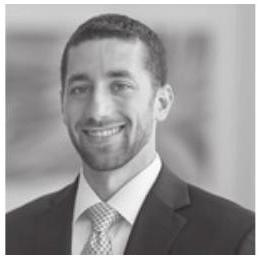
\includegraphics[max width=\textwidth, alt={}, center]{3c87ead7-70d5-42cb-a3a2-ed4cbdde9fd3-14_260_261_232_1078}

James Dallas received the B.S. degree from the Pennsylvania State University, University Park, PA USA, and the M.S. degree from the University of Michigan, Ann Arbor, MI USA, in 2017 and 2018, respectively, all in Mechanical Engineering. He is currently pursuing a Ph.D. in Mechanical Engineering with the University of Michigan. His research interests include modeling, system identification, system dynamics and control, and adaptive and robust optimal control, with applications to vehicle systems.

Michael P. Cole is a Mechanical Engineer in the\\
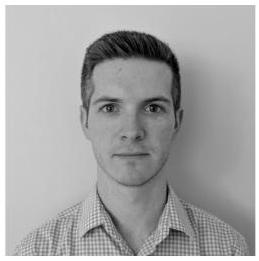
\includegraphics[max width=\textwidth, alt={}, center]{3c87ead7-70d5-42cb-a3a2-ed4cbdde9fd3-14_261_259_807_1078}\\
Dynamics and Mobility Modeling and Simulation branch within the Analytics division of the US Army Combat Capabilities Development Command (DEVCOM) Ground Vehicle Systems Center (GVSC). He serves as a co-lead for the Automotive Research Center (ARC) Thrust Area 1: Vehicle Dynamics, Control, and Autonomous Behavior and has worked in the areas of multibody dynamics, modeling and simulation, track and suspension, and engineering design. His research areas of interest include vehicle autonomy, vehicle dynamics, off-road mobility, and automation for wheeled and tracked military vehicles. He received his BSc in Mechanical Engineering from Wayne State University.\\
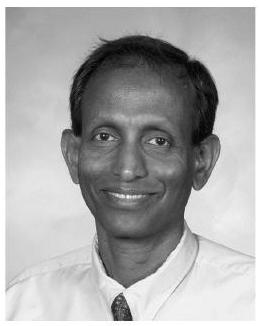
\includegraphics[max width=\textwidth, alt={}, center]{3c87ead7-70d5-42cb-a3a2-ed4cbdde9fd3-14_326_261_1443_1078}

Paramsothy Jayakumar received his M.S. and Ph.D. degrees in structural dynamics from Caltech, and B.S.E. degree from the University of Peradeniya, Sri Lanka. He is a Senior Technical Expert in Modeling and Simulation, SAE Fellow, and a member of the Analytics Team at the U.S. Army Ground Vehicle Systems Center in Warren, Michigan. Dr. Jayakumar is a member of the U.S. Army Acquisition Corps, an Honorary Fellow of the Department of Mechanical Engineering at the University of Wisconsin Madison, an Associate Editor for the ASME Journal of Computational and Nonlinear Dynamics, an Editorial Board Member for the International Journal of Vehicle Performance and the Journal of Terramechanics.\\
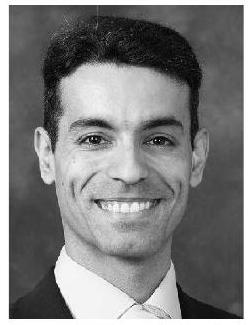
\includegraphics[max width=\textwidth, alt={}, center]{3c87ead7-70d5-42cb-a3a2-ed4cbdde9fd3-14_325_248_2114_1082}

Tulga Ersal received the B.S.E. degree from the Istanbul Technical University, Istanbul, Turkey, in 2001, and the M.S. and Ph.D. degrees from the University of Michigan, Ann Arbor, MI USA, in 2003 and 2007, respectively, all in mechanical engineering. He is currently an Associate Research Scientist in the Department of Mechanical Engineering, University of Michigan, Ann Arbor, MI. His research interests include modeling, simulation, and control of dynamic systems, with applications to vehicle and energy systems. Dr. Ersal is a member\\
of the ASME.


\end{document}